\documentclass[output=paper,colorlinks,citecolor=brown]{langscibook} 
\ChapterDOI{10.5281/zenodo.19708147}

\author{Alexandre François\affiliation{LaTTiCe, CNRS‒ENS-PSL, USN\\Australian National University}}
\title{Explicit apprehensions, implicit instructions: An indirect speech act in~the~grammar}
\abstract{Among the languages that grammaticalize the apprehensive domain, some use a~subordi\-nator like English\ \textit{lest} (`Don't run, \textit{lest} you fall'); others have an apprehensive mood in their verb system ($\approx$~`Don't run, you \textit{might} fall!'). The Oceanic languages of north Vanuatu, whose apprehensional strategies are quite diverse, feature both strategies. This study will focus on Mwotlap and its apprehensive mood. This modal marker appears to imply a form of interclausal dependency; yet rather than being due to syntactic subordination, this dependency effect is arguably pragmatic in nature. Indeed, by exposing an event as a risk to be avoided (e.g.\ `you might fall'), the apprehensive clause serves to justify a certain request (`don't run'). Sometimes, only the apprehension is made explicit (`You might fall!'), leading the hearer to reconstruct the intended order. The apprehensive mood thus reflects the grammaticalization of an indirect speech act: one where explicit apprehensions can stand for implicit instructions. The pragmatic effect \mbox{created} by this indirect request is sometimes exploited for politeness strategies, or for its humorous potential.}

%move the following commands to the "local..." files of the master project when integrating this chapter
%\usepackage{tabularx}
%\usepackage{langsci-optional}
%\usepackage{langsci-gb4e}
%\usepackage[tone]{tipa}

%\newcommand{\orcid}[1]{}

\IfFileExists{../localcommands.tex}{
   \addbibresource{../localbibliography.bib}
   \usepackage{tabularx,multicol}
\usepackage{url}
\urlstyle{same}

\usepackage{langsci-optional}
\usepackage{langsci-lgr}
\usepackage{langsci-gb4e}

\babelprovide[import]{hebrew}

\usepackage{paralist} %%may not be needed, currently used in questionnaire


%Siena added packages for introduction; not sure they are needed
\usepackage[normalem]{ulem}
\useunder{\uline}{\ul}{}

%from Treis:
\usepackage{listings}
\lstset{basicstyle=\ttfamily,tabsize=2,breaklines=true}

%%from Francez
% % % \usepackage{cjhebrew}
%\usepackage{tipa}  Also included by D&A, need to check with LSP whether to change it to language science tipa
\usepackage{leipzig}
%%from Dabkowski&AnderBois:

\usepackage[shortlabels]{enumitem} 
\usepackage{centernot}
\usepackage{arydshln}
\usepackage{newunicodechar}
\usepackage{csquotes}
%\let\sups\relax \usepackage{tipa} commented out on 7/3/25 Martina
% \usepackage[all]{nowidow}
\usepackage{listings} \lstset{basicstyle=\ttfamily}
\usepackage{multirow}
\usepackage{rotating}
\usepackage{pdflscape}
\usepackage{xspace}
%\usepackage{tabularx}
%\usepackage{multicol}
\usepackage{supertabular}
\usepackage{hhline}
\usepackage{bbding} %this package is for the checkmarks in Table 6 in Browne et al.

%\usepackage{qtree}
%\usepackage{tree-dvips}

\usepackage{array}
\usetikzlibrary{calc,tikzmark,matrix}
\usepgflibrary{shadings}
\usepackage{pifont}
%from Fedotov:

\usepackage{langsci-textipa}
%\usepackage{multirow}


%\usepackage{xeCJK}

%%%%%%%%%%%%%%%%%%%%%%%%%%%%%%%%%%%%%%%%%%%%%%%%%%%%
%%% EXAMPLES %%%%%%%%%%%%%%%%%%%%%%%%%%%%%%%%%%%%%%%
%%%%%%%%%%%%%%%%%%%%%%%%%%%%%%%%%%%%%%%%%%%%%%%%%%%% 

% if you want the source line of examples to be in
% italics, uncomment the following line
\renewcommand{\exfont}{\itshape}
% to add additional information to the right of
% examples, uncomment the following line

%\usepackage{langsci/styles/jambox}


%%% FOOTNOTE EXAMPLE NUMBERING
% \makeatletter
% \patchcmd{\@footnotetext}{\setcounter{fnx}{0}}{\renewcommand{\thexnumi}{\roman{xnumi}}}{}{}
% \apptocmd{\@footnotetext}{
%     \@noftnotetrue
%     \renewcommand{\thexnumi}{\arabic{xnumi}}%
% }{}{}
%
% \makeatother
\usepackage[linguistics,edges]{forest}
\usepackage{hyphenat}
\usepackage{langsci-branding}

   \makeatletter
\let\thetitle\@title
\let\theauthor\@author
\makeatother

\newcommand{\togglepaper}[1][0]{
   \bibliography{../localbibliography}
   \papernote{\scriptsize\normalfont
     \theauthor.
     \titleTemp.
    To appear in:
    Martina Faller,  Marine Vuillermet \&  Eva Schultze-Berndt (eds.). Apprehensional Constructions in a cross-linguistic perspective. Berlin: Language Science Press. [preliminary page numbering]
   }
   \pagenumbering{roman}
   \setcounter{chapter}{#1}
   \addtocounter{chapter}{-1}
}

\newbool{bookcompile}
\booltrue{bookcompile}
\newcommand{\bookorchapter}[2]{\ifbool{bookcompile}{#1}{#2}}


\newfontfamily\FedotovBoldEmptySetFont{LibertinusSerif-Italic.otf}[AutoFakeBold=2.5]
\newcommand{\FedotovBoldEmpty}{{\FedotovBoldEmptySetFont\bfseries ∅}}

%From Dabkowski&AnderBois


\let\sc\scshape
\let\rm\rmfamily
%\let\it\itshape
\let\tt\ttfamily
\let\nr\normalfont

\newcommand{\wsc}[1]{\textls[80]{\scshape#1}}

\let\textai\textit
% \let\textlc\spacedlowsmallcaps
% \let\textac\spacedallcaps
\let\textlc\textsc
\let\textac\textsc


%%%%%%%%%%%%%%%%%%%%%%%%%%%%%%%%%%%%%%%%%%%%%%%%%%%%
%%% FLAG %%%%%%%%%%%%%%%%%%%%%%%%%%%%%%%%%%%%%%%%%%%
%%%%%%%%%%%%%%%%%%%%%%%%%%%%%%%%%%%%%%%%%%%%%%%%%%%%

% \newcommand{\scott}  [1]{\textcolor{violet}{#1}}
% \newcommand{\maks}   [1]{\textcolor{blue}{#1}}
% % \newcommand{\data}   [1]{\textcolor{teal}{#1}}
% \newcommand{\new}   [1]{#1}
% \newcommand{\newnew}   [1]{\textcolor{teal}{#1}}
% \newcommand{\rev}   [1]{\textcolor{magenta}{#1}}



%%%%%%%%%%%%%%%%%%%%%%%%%%%%%%%%%%%%%%%%%%%%%%%%%%%%
%%% TABLES %%%%%%%%%%%%%%%%%%%%%%%%%%%%%%%%%%%%%%%%%
%%%%%%%%%%%%%%%%%%%%%%%%%%%%%%%%%%%%%%%%%%%%%%%%%%%%

%\newcolumntype{Y}{>{\arraybackslash}p{25.3543464286pt}} % length of L

% \newcolumntype{K}{>{\arraybackslash}p{24.25pt}}
% \newcolumntype{V}{>{\arraybackslash}p{(\textwidth/9-24pt)/2}}
%
\let\ch\relax \newcommand{\ch}[2]{\multicolumn{#1}{c}{\sc#2}}
\let\sx\relax \newcommand{\sx}[2]{\multicolumn{#1}{l}{\emph{-#2}}} % suffix
\let\su\relax \newcommand{\su}{\sx{1}} % suffix unicolumnal
\let\sd\relax \newcommand{\sd}{\sx{2}} % suffix dicolumnal
\let\cx\relax \newcommand{\cx}[2]{\multicolumn{#1}{l}{\emph{=#2}}} % clitic
\let\cu\relax \newcommand{\cu}{\cx{1}} % clitic unicolumnal
\let\cd\relax \newcommand{\cd}{\cx{2}} % suffix dicolumnal
\let\gx\relax \newcommand{\gx}[2]{\multicolumn{#1}{l}{\sc #2}} % gloss
\let\gd\relax \newcommand{\gd}{\gx{2}} % gloss dicolumnal
\let\gr\relax \newcommand{\gr}[1]{\multicolumn{2}{c}{\multirow{2}{*}{\textcolor{gray}{\sc#1}}}}
\let\db\relax \newcommand{\db}[1]{\multicolumn{2}{c}{\multirow{2}{*}{\sc#1}}}



%%%%%%%%%%%%%%%%%%%%%%%%%%%%%%%%%%%%%%%%%%%%%%%%%%%%
%%% EXAMPLES %%%%%%%%%%%%%%%%%%%%%%%%%%%%%%%%%%%%%%%
%%%%%%%%%%%%%%%%%%%%%%%%%%%%%%%%%%%%%%%%%%%%%%%%%%%%

%%% AFFIX BOUNDARY %%%%%%
% \DeclareRobustCommand{\longmn}{\textminus}
% \DeclareRobustCommand{\mn}{-}

%%% CLITIC BOUNDARY %%%%%%
% \DeclareRobustCommand{\longeq}{=}
% \makeatletter\DeclareRobustCommand{\eq}{%
%     \settowidth{\@tempdima}{-}% width of a hyphen
%     \resizebox{\@tempdima}{\height}{=}%
% }\makeatother

%%% FUZZY CLITIC %%%%%%
% \DeclareRobustCommand{\longfc}{%
%     $\overset{\text{\smash{}}}{\text{$\approx$}}$%
% }
% \makeatletter\DeclareRobustCommand{\fc}{%
%     \settowidth{\@tempdima}{-}% width of a hyphen
%     \resizebox{\@tempdima}{\height}{%
%         $\overset{\text{\smash{}}}{\text{$\approx$}}$%
%     }%
% }\makeatother

%%% REDUPLICATION %%%%%%%
% \DeclareRobustCommand{\longtl}{$\sim$}
% \makeatletter\DeclareRobustCommand{\tl}{%
%     \settowidth{\@tempdima}{-}% width of a hyphen
%     \resizebox{\@tempdima}{\height}{$\sim$}%
% }\makeatother

% \newcommand{\mn}          {\textminus}
\newcommand{\src}    [1]  {\jambox[0pt]{\rm(#1)}}
% \newcommand{\ai}     [2]  {\emph{#1} `\textsc{#2}#3'\xspace}
\newcommand{\ai}     [2]  {\emph{#1} `\textsc{#2}'\xspace}
\newcommand{\sane}   [1][]{\ai{=sa'ne}{appr}{#1}}
\newcommand{\srcn}   [1][]{\ai{kûintsû}{srcn}{#1}}
% \newcommand{\mbekane}[1][]{\ai{\eq mbe kañe}{neg.adv aux.inf}{#1}}

% \let\sc\relax \newcommand{\sc}{\normalfont\scshape}
% \let\rm\relax \newcommand{\rm}{\normalfont\rmfamily}
% \let\it\relax \newcommand{\it}{\normalfont\itfamily}

\newcommand{\lb}{{\rm[}}
\newcommand{\rb}{{\rm]}}

\newcommand{\bad}{\makebox[0pt][r]{*\,}}
\newcommand{\infel}{\makebox[0pt][r]{\#\,}}


% \newcommand{\lsqz}[1]{#1}
% \newcommand{\lsqz}[1]{\makebox[0pt][l]{#1}}

% \newcommand{\lsqu}[1]{\makebox[0pt][l]{#1}}
% \newcommand{\rsqu}[1]{\makebox[0pt][r]{#1}}
% \newcommand{\astr}{\makebox[0pt][r]{{\nr*}}}
% \newcommand{\hash}{\makebox[0pt][r]{{\nr\#}}}
% \newcommand{\qstn}{\makebox[0pt][r]{{\nr?}}}
% \newcommand{\bad}{\makebox[0pt][r]{*}}
% \newcommand{\unhappy}{\makebox[0pt][r]{\#}}


%%%%%%%%%%%%%%%%%%%%%%%%%%%%%%%%%%%%%%%%%%%%%%%%%%%%
%%% UNICODE CHARACTERS  %%%%%%%%%%%%%%%%%%%%%%%%%%%%
%%%%%%%%%%%%%%%%%%%%%%%%%%%%%%%%%%%%%%%%%%%%%%%%%%%%

\newunicodechar{⟨}{⟨}
\newunicodechar{⟩}{⟩}

\newcommand{\infix}{⟨}
\newcommand{\outfix}{⟩}



%%%%%%%%%%%%%%%%%%%%%%%%%%%%%%%%%%%%%%%%%%%%%%%%%%%%
%%% IPA %%%%%%%%%%%%%%%%%%%%%%%%%%%%%%%%%%%%%%%%%%%%
%%%%%%%%%%%%%%%%%%%%%%%%%%%%%%%%%%%%%%%%%%%%%%%%%%%%

% \newcommand{\ipa}{\textipa}

\newcommand{\sub}{\textsubscript}
% \let\super\relax \newcommand{\super}{\textsuperscript}

\newcommand{\ts}{\texttslig}
% \let\dz\relax \newcommand{\dz}{\textdzlig}
\newcommand{\tS}{\textteshlig}
\newcommand{\dZ}{\textdyoghlig}
\newcommand{\cj}{\textctc}
\newcommand{\sj}{\textctc}
\newcommand{\zj}{\textctz}
\newcommand{\tcj}{\texttctclig}
\newcommand{\tsj}{\texttctclig}
\newcommand{\dzj}{\textdctzlig}
\newcommand{\gj}{\textbardotlessj}
% \let\nj\relax \newcommand{\nj}{\textltailn}
% \newcommand{\W}{\textturnmrleg}
\newcommand{\wl}{\textturnmrleg}
% \newcommand{\1}{\ipabar{\~\i}{.5ex}{1.1}{}{}}
\newcommand{\dotlessibar}{\ipabar{\i}{.5ex}{1.1}{}{}}
\newcommand{\darkl}{\textltilde}
% \newcommand{\n}{\textsubarch}
% \newcommand{\x}{\textovercross}
\newcommand{\lowered}{\textlowering}
\newcommand{\raised}{\textraising}
\newcommand{\retracted}{\textsubbar}
\newcommand{\unreleased}{\textcorner}
% \newcommand{\syllabic}{\s}
\newcommand{\implosivet}{\texthtt}
\newcommand{\implosived}{\texthtd}
\newcommand{\implosivep}{\texthtp}
\newcommand{\implosiveb}{\texthtb}
\newcommand{\implosivek}{\texthtk}
\newcommand{\implosiveg}{\texthtg}



%%%%%%%%%%%%%%%%%%%%%%%%%%%%%%%%%%%%%%%%%%%%%%%%%%%%
%%% OTHER %%%%%%%%%%%%%%%%%%%%%%%%%%%%%%
%%%%%%%%%%%%%%%%%%%%%%%%%%%%%%%%%%%%%%%%%%%%%%%%%%%%

\newcommand{\ie}{i.\,e.\xspace}
\newcommand{\Ie}{I.\,e.\xspace}
\newcommand{\eg}{e.\,g.\xspace}
\newcommand{\Eg}{E.\,g.\xspace} 




\newcommand{\francoissource}[1]{\hfill\textnormal{{\footnotesize #1} }}
\newcommand{\E}{Ɛ\kern-1.5pt\raisebox{1pt}{̏}\kern1.5pt}
\newcommand{\ù}{{ṵ}\kern-2pt{̀}\kern2pt}
\newcommand{\ȕ}{{ṵ}\kern-2pt{̏}\kern2pt}

\newcommand{\OO}{ɔ\kern-1pt\raisebox{-1pt}{̰}\kern1pt}
\newcommand{\Ǒ}{{{ɔ̌\kern-1pt\raisebox{-.5pt}{̰}\kern1pt}}}


\newcommand{\à}{{a̰}\kern-2pt{̀}\kern2pt}
\newcommand{\ilit}[1]{#1\il{#1}}

   %% hyphenation points for line breaks
%% Normally, automatic hyphenation in LaTeX is very good
%% If a word is mis-hyphenated, add it to this file
%%
%% add information to TeX file before \begin{document} with:
%% %% hyphenation points for line breaks
%% Normally, automatic hyphenation in LaTeX is very good
%% If a word is mis-hyphenated, add it to this file
%%
%% add information to TeX file before \begin{document} with:
%% %% hyphenation points for line breaks
%% Normally, automatic hyphenation in LaTeX is very good
%% If a word is mis-hyphenated, add it to this file
%%
%% add information to TeX file before \begin{document} with:
%% \include{localhyphenation}

\hyphenation{
par-a-digm
com-ple-men-ta-tion
anaph-o-ra
Dor-drecht
Cu-shi-tic
be-ne-dic-tive
pa-ra-digms
Ethi-o-pi-an
hoch-land-ost-ku-schi-ti-schen 
Duu-raa-me
Pa-ken-dorf
Lich-ten-berk
affri-ca-te
affri-ca-tes
com-ple-ments
Eng-lish
}




\hyphenation{
par-a-digm
com-ple-men-ta-tion
anaph-o-ra
Dor-drecht
Cu-shi-tic
be-ne-dic-tive
pa-ra-digms
Ethi-o-pi-an
hoch-land-ost-ku-schi-ti-schen 
Duu-raa-me
Pa-ken-dorf
Lich-ten-berk
affri-ca-te
affri-ca-tes
com-ple-ments
Eng-lish
}




\hyphenation{
par-a-digm
com-ple-men-ta-tion
anaph-o-ra
Dor-drecht
Cu-shi-tic
be-ne-dic-tive
pa-ra-digms
Ethi-o-pi-an
hoch-land-ost-ku-schi-ti-schen 
Duu-raa-me
Pa-ken-dorf
Lich-ten-berk
affri-ca-te
affri-ca-tes
com-ple-ments
Eng-lish
}



   \boolfalse{bookcompile}
   \togglepaper[23]%%chapternumber
}{}

\begin{document}
\maketitle

\shorttitlerunninghead{Explicit apprehensions, implicit instructions}%%use this for an abridged title in the page headers

\section{Are apprehensional constructions inherently dependent?}
\label{sec:1}

\subsection{Apprehensional constructions: Presentation}
\label{subsec:acpresentation}

The grammatical encoding of apprehensional meanings was initially brought to light in individual language descriptions, covering various families and areas -- e.g.\ \citet{Austin1981} on \ili{Diyari} (\ili{Pama-Nyungan}, Australia); \citet{lichtenberk1995} on Toqa\-ba\-qita (\ili{Oceanic}, Solomons); \citet{francois2003} on \ili{Mwotlap} (\ili{Oceanic}, Vanuatu); \citet{pakendorfschalley2007} on \ili{Sakha} (\ili{Turkic}, Siberia); \citet{vuillermet2018a} on \ili{Ese Ejja} (\ili{Takanan}, Bolivia/Peru); \citet{smithdennis2021} on \ili{Papapana} (\ili{Oceanic}, Papua New Guinea) -- to cite but a few. Beyond the discrepancies in terminology and glossing (``avertive'', ``evitative'', ``apprehensive'', ``adversative'', \textit{lest}  {\ldots}), these various constructions appear to share enough properties to justify defining a new semantic domain, label\-led \textit{apprehensional}. This has led to a recent line of research in typology (see \citealt{Dobrushina2006,  vuillermet2018b, vuillermet2018a, fallerschultzeberndt2018}) -- and is the~object of the present volume.


In a nutshell, apprehensional markers are grammatical morphemes that label a potential event as undesirable, and worthy of being avoided indirectly -- by carrying out another action. Whereas prohibitives (such as \textit{Don't jump!}) ask the addressee to directly refrain from an action (assuming they can control it), the semantic mechanism of an apprehensive is more complex, because it normally involves two distinct events P and Q: an event P which can be controlled, and a second event Q which cannot be controlled directly, but which can be avoided, by carrying out the action~P.

Here is an example from the \ili{Oceanic} language \ili{Papapana} (Papua New Guinea) as described by \citet{smithdennis2021}:


 
\ea \langinfo{Papapana}{\ili{Oceanic}; Papua New Guinea}{\citealt[426]{smithdennis2021}} \\
\label{ex:Fra1}
\gll O=nabe=i, o=\textbf{te} mate=i. \\
\textsc{2sg.sbj}=swim=\textsc{irr} \textsc{2sg.sbj=\textbf{appr}} die=\textsc{irr} \\
\glt `Swim, (otherwise) you might die.' \textasciitilde~`Swim, (so that) you don't die.' 
\z
 
\noindent In this example, the undesirable event (Q) is \{you dying\}, over which the addressee has no direct control. So, instead of asking them to avoid Q directly by means of a prohibitive (*\textit{Don't die!}), the speaker requests that Q be avoided \textit{indirectly} -- namely, by carrying out another action P (\textit{Swim!}) which should prevent Q from happening. In such a structure, the apprehensive clause (\textit{you might die}) serves as a justification for the main clause (\textit{Swim!}): it clarifies the nature of the undesirable event Q that this action P should help avoid.
 

\subsection{Two main apprehensional strategies}
\label{subsec:twomain}

 
The typological characteristics of the apprehensional domain are explained in this volume's introduction (\citealt{chapters/introduction}); I will only mention a few points, using the same terminology as them. 

Apprehensional morphemes may belong formally to two main grammatical types: (a) a subordinating conjunction, or (b) a modal marker on the predicate.



Apprehensional subordinators (e.g.\ \ili{English} \textit{for fear that}) encode an undesirable event as a dependent clause Q, which serves as an explanation for the main clause P. The typical structure, labelled ``precautioning'' (\citealt[260]{vuillermet2018a}, \citealt{chapters/introduction}), takes the form of a twofold structure {\{P,~\textsc{sub}~Q\}}. P is called a ``pre-emptive clause'', whether it encodes an order, a prohibition, or a statement. As for the undesirable situation Q that is meant to be avoided through the event P, it is called the ``precautioning clause''. In \ili{English}, this can be rendered using the (archaic) subordinator \textit{lest}:

\ea \label{ex:Fra2a}
\textnormal{\{}I put the knife away\textnormal{\}}\textnormal{\textsc{\textsubscript{p}}} \textnormal{\{}\textbf{\textit{lest}} you hurt yourself\textnormal{\}}\textnormal{\textsc{\textsubscript{q}}}.
\z

\noindent In principle (though there can be exceptions), such subordinators are restricted to dependent clauses, and never occur in main clauses.

The second major formal strategy involves a special modal marker on the verb, labelled the ``apprehensive mood'' \citep{chapters/introduction}. As a first approximation, the apprehensive mood can be rendered in \ili{English} with the modal auxiliary \textit{might}. This can also surface as a twofold structure \{P, \textsc{mod} Q\} -- mostly parallel to (\ref{ex:Fra2a}) above:
 
\ea \label{ex:Fra2b}
    \textnormal{\{}I put the knife away\textnormal{\}\textsc{\textsubscript{p}}}, {\op}\textit{because}{\cp}  \textnormal{\{}you \textbf{\textit{might}} hurt yourself\textnormal{\}\textsc{\textsubscript{Q}}}.
\z
 
One key difference between the subordinating strategy and the modal one is that the latter can also be used in an independent clause:
 
\ea \label{ex:Fra2c}
You \textbf{\textit{might}} hurt yourself.
\z

\noindent A sentence like (\ref{ex:Fra2c}) may be syntactically well-formed, but it typically implies a reference to an intended instruction (order, prohibitive) which is either explicit, or must be inferred from the context. This question will be central to our study.

Languages differ in their degree of grammaticalization of apprehensional strategies. The reason why it took a long time to identify this domain as typologically significant is that many of the world's languages use linguistic devices that do not target that meaning specifically. For example, while \ili{English} \textit{might} can sometimes be interpreted as the equivalent of an apprehensive mood as in (\ref{ex:Fra2b}), this auxiliary has a broader semantic spectrum, which is not restricted to undesirable events (cf.\ \textit{You might be able to find a good job there}). Yet more and more languages are being found to feature grammaticalized morphemes whose role is specifically to tag events as undesirable. 

Most languages have only one of the two strategies described above, either the precautioning subordinator or the apprehensive mood. \ili{Ese Ejja} is noteworthy in having both: a subordinator \textit{e-\ldots kwajejje} and an apprehensive \textit{\nobreakdash-chana} \citep{vuillermet2018a} -- corresponding, respectively, to structures like (\ref{ex:Fra2a}) and (\ref{ex:Fra2b})--(\ref{ex:Fra2c}) above. Finally, some languages have a single morpheme (like \textit{ada} in Toqa\-baqita, \citealt{lichtenberk1995}) that can fill both functions, subordinating and main-clause modal.
 

\subsection{Apprehensive mood and clause dependency in northern Vanuatu}
\label{subsec:moodandclause}

 
The present study aims to describe and compare the apprehensional strategies of a group of 17 \ili{Oceanic} languages spoken in the Torres and Banks Islands of north Vanuatu. In spite of their historical diversification, these related languages are often structurally parallel \citep{François2011}: one of their commonalities is precisely to have grammaticalized strategies to encode apprehensional semantics.

However, what is also striking is the diversity of these devices: not only do the morphemes differ in their form, but they also result from different paths of grammaticalization. Some only have a ‘lest’ subordinator, others only an apprehensive mood, others have both. After an overview of the strategies attested in the region (\sectref{sec:apprehensionalsemantics}), the second half of this study will focus on the language \ili{Mwotlap}, which employs a modal marker \textit{tiple}:\footnote{Examples are cited in their practical orthographies. Conventions for \ili{Mwotlap} include:  \textit{e} = [{ɛ}]; \textit{ē} = [{ɪ}]; \textit{o} = [{ɔ}]; \textit{ō} = [{ʊ}]; \textit{y} = [{j}]; \textit{g} = [{ɣ}]; \textit{b} = [{ᵐb}]; \textit{d} = [{ⁿd}]; \textit{\={n}} = [{ŋ}]; \textit{q} = [{k͡pʷ}]; \textit{\={m}} = [{ŋ͡mʷ}]. Other languages of the area essentially share the same conventions.}
 
\ea \label{ex:Fra3} \textnormal{Mwotlap}\\
\gll ${\langle}$Tēy van na-gayga en,${\rangle}$\textnormal{\textsc{\textsubscript{p}}} ${\langle}$nēk \textbf{tiple} qēsdi${\rangle}$\textnormal{\textsc{\textsubscript{q}}}! \\
hold \textsc{direc} \textsc{art}-rope \textsc{def} \textsc{2sg} \textsc{appr} fall \\
\glt `Hold on to the rope, (otherwise) you \textit{might} fall! / \textit{lest} you fall!'
\z
 
\noindent The form \textit{tiple} fits in the slot of Tense-Aspect-Mood markers in \ili{Mwotlap}, and will thus be described as its ``apprehensive mood'' (\citealt[130]{François2005a}).

Parallel to (\ref{ex:Fra2b}) above, \ili{Mwotlap} \textit{tiple} is most often found in biclausal sentences such as (\ref{ex:Fra3}); this can make it functionally equivalent to a subordinate structure of the type \{P, \textit{lest} Q\}. As~it~happens, northern Vanuatu is an area where certain Tense-Aspect-Mood markers have been observed to encode, by themselves, a form of clause dependency (\sectref{subsec:juxtaposed}). Could it be the case that the apprehensive mood of \ili{Mwotlap} also encodes syntactic subordination on its own?

In fact, it is not rare to hear utterances consisting only of an apprehensive clause Q, with no pre-emptive clause P:
 
\ea \label{ex:Fra4}
\gll Nēk \textbf{tiple} qēsdi! \\
\textsc{2sg} \textsc{\textbf{appr}} fall \\
\glt [\textit{to a boy in a tree}] `Hey, you might fall!'
\z

 Such examples raise the question of the status of that sentence: is it fully independent? Or is it dependent in some way, either syntactic or pragmatic? This is indeed a recurring question in the typology of apprehensional constructions:

\begin{quote}
    ``One of the main issues in the existing literature on apprehensives is their syntactic and/or pragmatic status as dependent or independent clauses.'' \citep[428]{smithdennis2021}
\end{quote}

The question thus arises of how best to analyze examples such as (\ref{ex:Fra4}). If~\textit{tiple} were found to have a subordinating role, then one may want to analyze a stand-alone clause like (\ref{ex:Fra4}) as an instance of \textit{insubordination} -- i.e.\ a subordinate clause used independently (cf.\ \citealt{evans_insubordination_2007}). Such a historical process has indeed been proposed to account for certain types of apprehensional markers, as in the \ili{Oceanic} language \ili{Papapana} \citep{smithdennis2021} or in the \ili{East Caucasian} language \ili{Archi} \citep{chapters/daniel}. Rather, I will propose that apprehensive clauses in \ili{Mwotlap} are grammatically well-formed independent sentences. They do present a form of dependency towards an external utterance, explicit or implicit; yet that dependency is not syntactic in nature, but rather pragmatic.

In the analysis I propose, the work of the apprehensive modality is to alert the addressee to a specific risk that should be avoided. By formulating such an apprehension, the speaker yields support to a particular instruction -- one that is sometimes specified as in (\ref{ex:Fra3}), and sometimes left implicit as in (\ref{ex:Fra4}). This interplay between \textit{explicit apprehensions} and \textit{implicit instructions} is the central mechanism of the apprehensive mood of \ili{Mwotlap}.



\subsection{Data and sources}
\label{subsec:dataandsources}

The present study rests on primary data I collected during a number of field trips in Vanuatu since 1997, on the 17 languages of the Torres and Banks Islands (see~Figure~\ref{fig:map1}). For reasons of length, this article will only mention a representative sample of eight languages: \ili{Hiw}, \ili{Lo-Toga}, \ili{Löyöp}, \ili{Lemerig}, \ili{Vurës}, \ili{Dorig}, \ili{Lakon} -- and of course, \ili{Mwotlap}. 


\begin{figure}
    \caption{Location of the 17 Torres and Banks languages in Vanuatu (South~Pacific)}
%     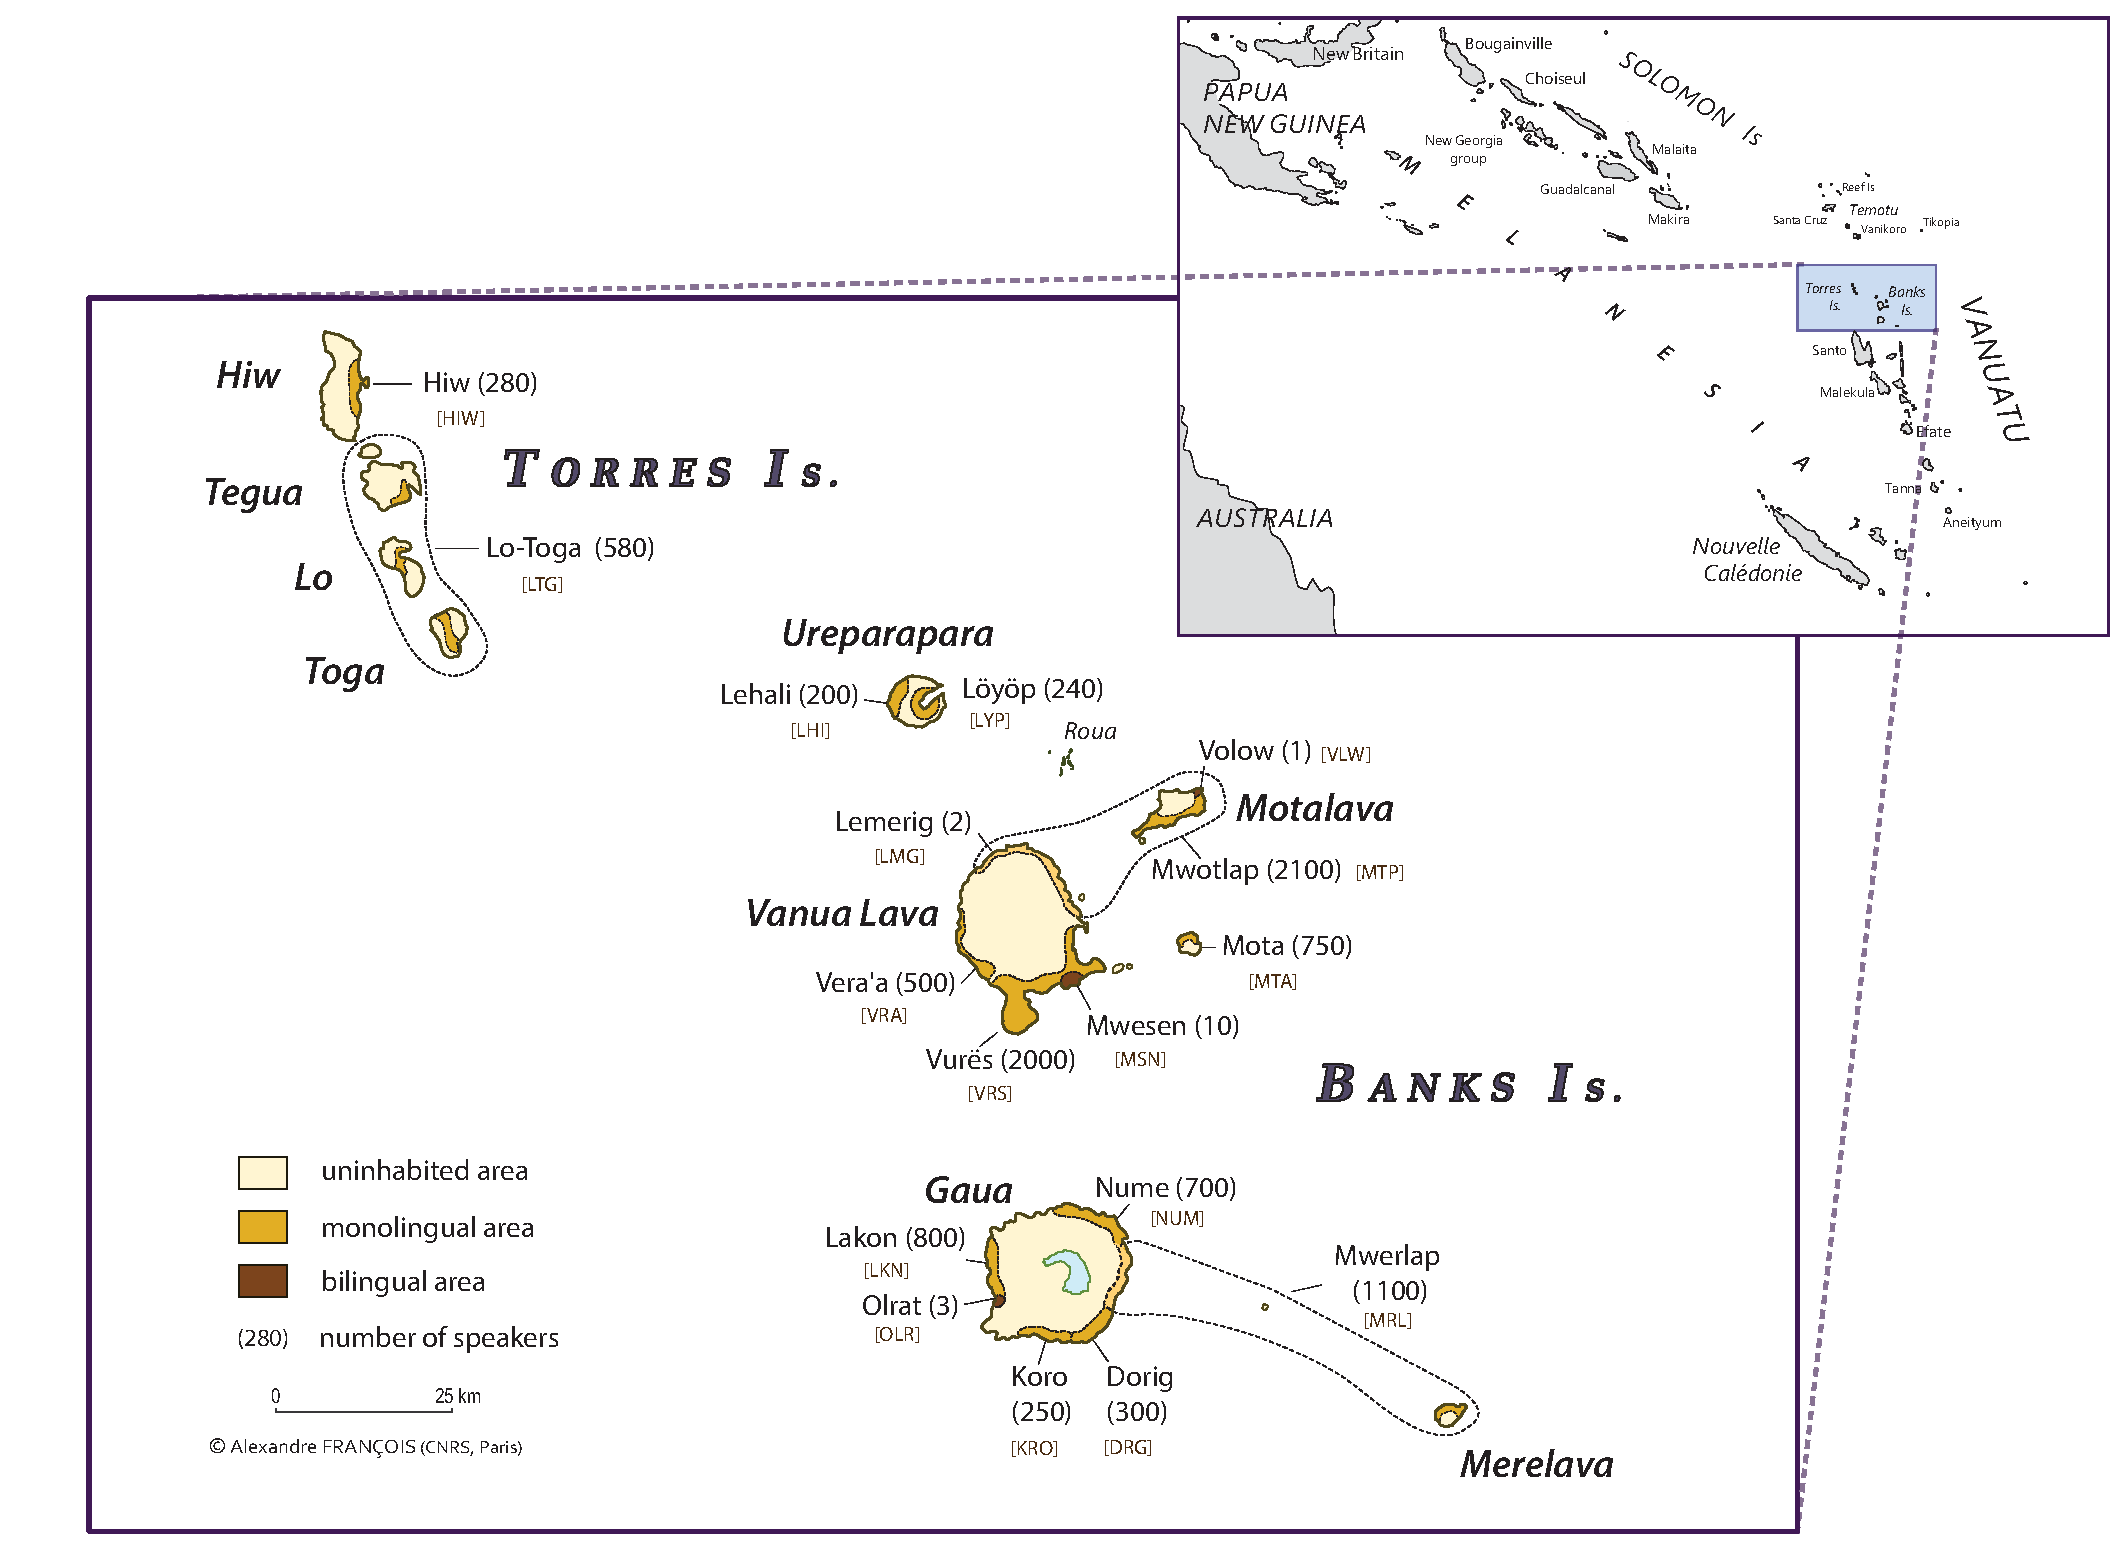
\includegraphics[width=1\textwidth]{figures/AlexFrancois_Vanuatu_Torres-Banks.eps}
    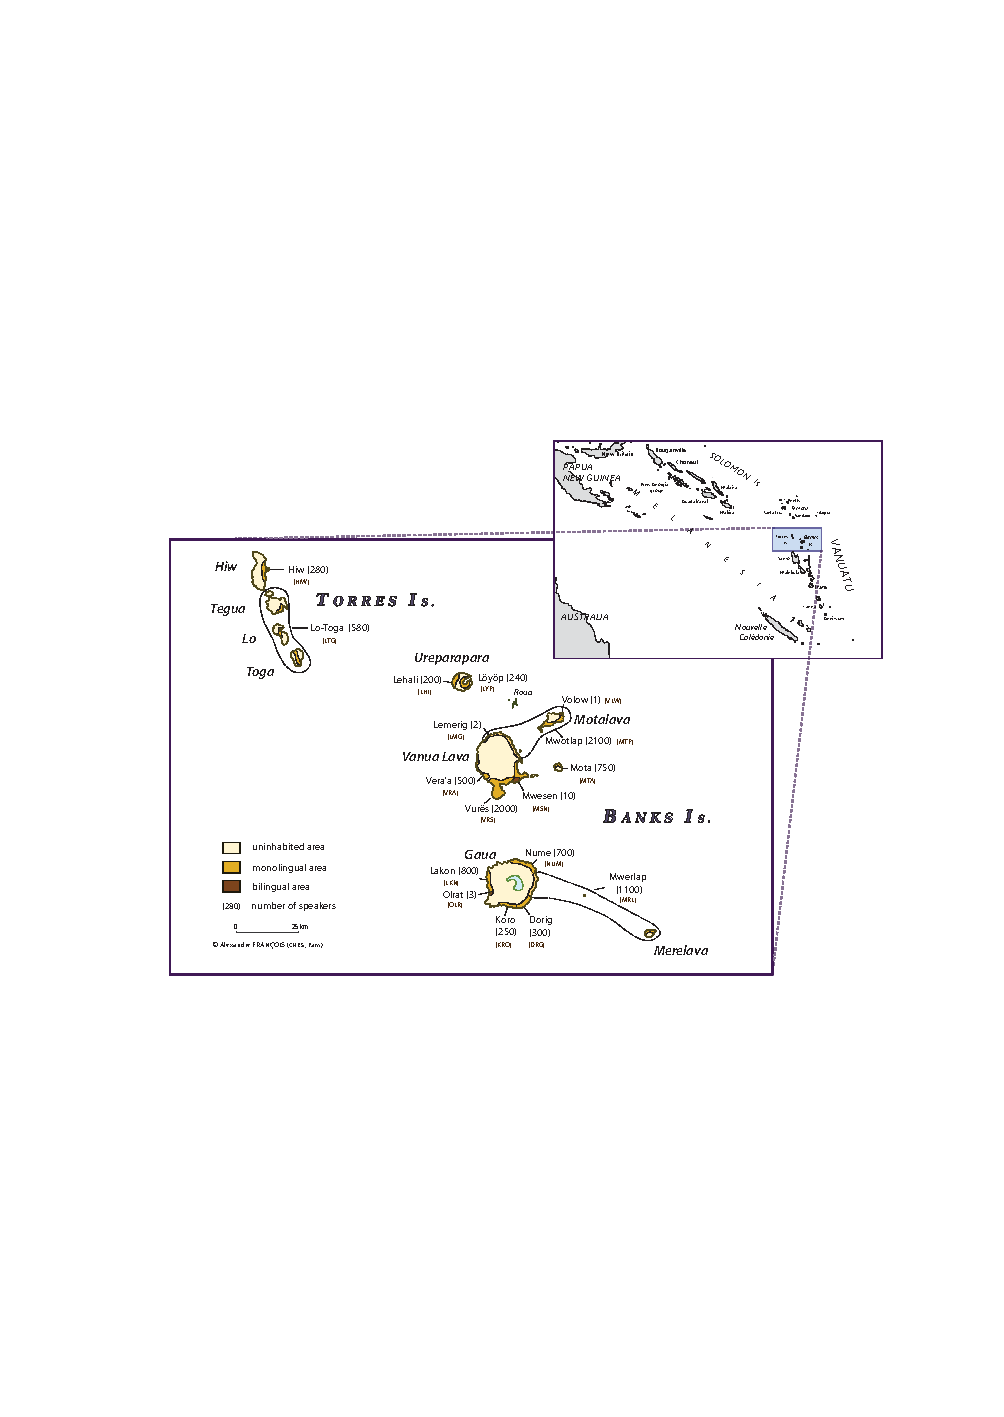
\includegraphics[width=1\textwidth]{figures/mapdorig.pdf}
    \label{fig:map1}
\end{figure}
My sources take the form of three main sets of data. First, I designed a conversational questionnaire \citep{François2019} aiming to elicit lexical, grammatical and phraseo\-logical data in each language: this allowed me to collect essential information on apprehensional structures from all 17 languages.\footnote{This questionnaire helped me elicit example sentences (\ref{ex:Fra17}), (\ref{ex:Fra20}), (\ref{ex:Fra21}), (\ref{ex:Fra27}) below.} Second, participant-observer immersion in each language community gave me the opportunity to collect snippets of spontaneous conversation in my handwritten notebooks (archived in \citealt{François2015}).

Finally, I recorded 389 narratives and conversations, totalling 50 hours, in all languages. Among these, 263 texts were transcribed and annotated in the presence of native speakers; together, they form an electronic text corpus of 250,000 words -- with the largest corpora being in \ili{Mwotlap} (100,000 w.), \ili{Lo-Toga}, \ili{Hiw}, \ili{Dorig}, \ili{Lakon}, \ili{Lemerig}. These recordings are all archived in the \textit{Pangloss Collection} of the CoCoON archive, with open access \citep{François2022a}. I regularly enrich them with time-aligned transcriptions and translations, which are indexed using permanent identifiers (\textsc{doi}) at the sentence level. 



The present study will cite examples either from my field notes or from my text corpora; whenever a sentence is accessible online, I~will provide a permanent link to it, so it can be heard in its original context. While apprehensional markers regularly surface in the spoken narratives I recorded, I was also able to hear many tokens in the spontaneous speech of daily conversations; in such cases -- arguably the most natural ones -- rather than links to audio files, I will provide references to my field notes.

Several linguists have worked on northern Vanuatu languages, whether their focus was the lexicon (\citealt{CodringtonPalmer1896} for \ili{Mota}; \citealt{Malau2021} for \ili{Vurës}; \citealt{François2022b} for \ili{Mwotlap}) or the grammar (\citealt{François2001,francois2003} for \mbox{Mwotlap}; \citealt{Schnell2011} for \ili{Vera'a}; \citealt{Malau2016} for \ili{Vurës}). An overview of the Torres and Banks languages can be found in \citet{François2011,François2012}. The present study finds its roots in my descriptive monograph on the Tense-Aspect-Mood system of \mbox{Mwotlap} \citep{francois2003}, particularly in the chapter ``Évitatif'' (pp.~301--312). However, I will bring here new insights and discussion, as well as a much greater amount of primary data -- in \ili{Mwotlap} and especially in the other languages, most of which are still undocumented.

This study will begin with an overview of apprehensive strategies in northern Vanuatu (\sectref{sec:apprehensionalsemantics}), highlighting their diversity, and their links with other grammatical devices (ablative case, prohibitive modality). We will then focus on the morpheme \textit{tiple} of \ili{Mwotlap}, as it shows the most unambiguous case of an apprehensive modality, distinct from other moods, and clearly different from a precautioning subordinator. After describing the syntax and semantics of the \ili{Mwotlap} apprehensive (\sectref{sec:moodmwotlap}), \sectref{sec:standalone} will return to our discussion about the stand-alone uses of the apprehensive -- as in (\ref{ex:Fra4}) above -- and to their pragmatic correlates.
 

\section{Apprehensional semantics in north Vanuatu}
\label{sec:apprehensionalsemantics}

\subsection{Grammatical overview of north Vanuatu languages}
\label{subsec:grammoverview}

 
The Vanuatu archipelago was first settled about 3,100 years ago by Austronesian navigators, speakers of the Proto \ili{Oceanic} language (\citealt{BedfordSpriggs2008}, \citealt{Lipsonetal2020}). This was followed by three millennia of \textit{in situ} diversification, during which the linguistic unity of Vanuatu progressively fragmented into 138 languages \citep{Françoisetal2015}. Among these, 17 formed in the northern islands of the Torres and Banks groups, through a process of internal diversification.

In spite of their divergence, the linguistic history of northern Vanuatu is also one of structural convergence, due to a sustained history of contact among communities \citep{François2011}. Today, the Torres and Banks languages share many linguistic structures -- whether this is due to their common origin, or to later re-convergence. 

The next paragraphs provide a short overview of some major grammatical properties common in the area, and relevant to the discussion of apprehensional strategies. (For the sake of internal consistency, all examples in this overview will be given in \ili{Mwotlap}.)




\subsubsection{Word order in the verbal clause}
\label{subsubsec:wordorder}

The languages of Vanuatu have accusative alignment. They have fixed rules for word order in the clause, with a consistent order SVO (i.e.\ SV, AVO):

\ea \label{ex:Fra5} \textnormal{Mwotlap}\francoissource{{[\url{https://doi.org/10.24397/pangloss-0007409\#S25}]}}\\
\gll Iplu-k mē-dē\={n} ēgēn. \\
partner-\textsc{1sg} \textsc{prf}-arrive now \\
\glt `My friend has arrived.' 
\z

    \ea \label{ex:Fra6} \textnormal{Mwotlap} \francoissource{{[\url{https://doi.org/10.24397/pangloss-0003282\#S76}]}}\\
\gll Gēn tu-wuh Vēnvēntey talōw. \\
\textsc{1incl.pl} \textsc{fut}-kill (V.) tomorrow \\
\glt `We will kill Vēnvēntey tomorrow.' 
\z

Subordinators, such as the complementizer, are normally found at the left edge of the dependent clause, before its subject:
 
    \ea \label{ex:Fra7} \textnormal{Mwotlap} \francoissource{{[\url{https://doi.org/10.24397/pangloss-0002298\#S73}]}}\\
\gll No ne-myōs \textbf{so} nok leg mi nēk. \\
\textsc{1sg} \textsc{stat}-want \textsc{\textbf{comp}} \textsc{1sg.irr} marry with \textsc{2sg} \\
\glt `I want to marry you.' 
\z


\noindent Independent and subordinate clauses have the same internal word order.



\subsubsection{Tense-Aspect-Mood-Polarity marking}
\label{subsubsec:tampmarking}

 
The syntax of verbal clauses revolves around a constituent which the \ili{Oceanic} tradition (e.g.\ \citealt{Durie1988}, \citealt{Evans2003}) calls the \textit{verb complex} (\textsc{vc}). 

The \textsc{vc} consists minimally of a verb, which is the head.\footnote{Lexical adjectives and nouns can also head predicates inflecting in \textsc{tamp}, in the same way as verbs do (\citeauthor{François2005a} \citeyear[131]{François2005a}, \citeyear[328]{François2017}, \citeyear{Françoisforthcomingb}). Thus, while most examples of apprehensives in this study will involve a verbal head, (\ref{ex:Fra33})--(\ref{ex:Fra34}) will involve adjectives, and (\ref{ex:Fra49}) a noun predicate.} This head is optionally followed by one or more postverbal modifiers: e.g.\ a second verb in a serial pattern, or a \textit{postverb} (a kind of adverb specialized in the postverbal position). In~(\ref{ex:Fra8}), the verb complex includes a verbal head \textit{van} `walk' and a postverb \textit{yeghuquy} `freely':
 
\ea \label{ex:Fra8} \textnormal{Mwotlap} \francoissource{{[\url{https://doi.org/10.24397/pangloss-0007411\#S123}]}}\\
\gll N-et ${\langle}$tit- \textbf{\textsc{van}} \textbf{yeghuquy} vēhte${\rangle}$\textnormal{\textsc{\textsubscript{vc}}} van lē-vētan en. \\
\textsc{art}-person \textsc{neg:pot\textsubscript{1}}- walk freely \textsc{neg:pot\textsubscript{2}} \textsc{direc} \textsc{loc}-land \textsc{def} \\
\glt `One cannot walk freely into that piece of land.' 
\z

Attached to the lexical elements of the verb complex are markers of Tense, Aspect, Mood, and Polarity (henceforth \textsc{tamp}), which take the form of affixes or particles. Example (\ref{ex:Fra8}) has a discontinuous \textsc{tamp} marker, the Negative potential \textit{tit-} {\ldots} \textit{vēhte} `cannot'. In Torres and Banks languages, \textsc{tamp} morphemes cannot combine with each other: they form a single paradigm of unanalyzable, portmanteau forms that encode the semantics of tense, aspect, mood, and polarity in a single morpheme -- whether it is simple or discontinuous. The \textsc{tamp} paradigm in \ili{Mwotlap} has 26 members (\citealt[133]{François2005a}), one of which is the apprehensive mood \textit{tiple} (\sectref{sec:moodmwotlap}).
 

 
\textsc{Tamp} morphemes occur in two slots in the clause, labelled \textsc{tamp\textsubscript{1}} and \textsc{tamp\textsubscript{2}}, which surround the lexical elements of the verb complex: 
 

\ea \label{ex:Fra9} \textnormal{Structure of a verbal clause in \ili{Mwotlap}: \\
\textit{subject} $\langle$ \textsc{tamp\textsubscript{1}} \textsc{Verb} (postverbs) \textsc{tamp\textsubscript{2}} $\rangle$\textsubscript{\textsc{vc}} \textit{object} adjuncts}
\z

\noindent One slot \textsc{tamp\textsubscript{1}} follows the subject, and opens the verb complex. The second slot \textsc{tamp\textsubscript{2}} closes it, preceding the object\footnote{\ili{Mwotlap} is strict in inserting \textsc{tamp\textsubscript{2}} before the object; other Torres and Banks languages sometimes place it after the object.} or any other complement. 

Some \textsc{tamp} morphemes are bipartite, with components occupying both slots \textsc{tamp\textsubscript{1}} and \textsc{tamp\textsubscript{2}}: this was illustrated in (\ref{ex:Fra8}) with the Negative potential \textit{tit-}\ldots\  \textit{vēhte}.\footnote{In these lines, the ellipsis ``\ldots'' corresponds to the lexical elements of the \textsc{vc} (i.e.\ the verb complex minus \textsc{tamp} markers). Bipartite morphemes include discontinuous morphemes of negation, which are common in Banks languages: see \citet[31]{Schnell2011} for \ili{Vera'a}, \citet{Françoisforthcominga} for \ili{Dorig}.} Some consist of a single element that occurs postverbally in \textsc{tamp\textsubscript{2}}. But the majority of \textsc{tamp} morphemes occupy only the first slot \textsc{tamp\textsubscript{1}} -- e.g.\ the Perfect  \textit{me-}\ldots\ in~(\ref{ex:Fra5}) or the Future \textit{te-}\ldots\ in~(\ref{ex:Fra6}). The Apprehensive \textit{tiple} also belongs in that \textsc{tamp\textsubscript{1}} slot -- as we saw in (\ref{ex:Fra4}).

\subsubsection{Subordination and \textsc{tamp}}
\label{subsubsec:subandtamp}

When two morphemes are homophonous, they can often be identified through their position in the sentence. 

For example, (\ref{ex:Fra10}) has a particle \textit{so} that is located between the subject and the verb, in the \textsc{tamp\textsubscript{1}} slot; therefore, it is a \textsc{tamp} marker. This is an instance of the \textit{prospective} mood, which encodes a number of irrealis values (volitional, deontic, hortative, subjunctive) in the affirmative (\citealt[134]{François2005a}):

\ea \label{ex:Fra10} \textnormal{Mwotlap} \francoissource{{[\url{https://doi.org/10.24397/pangloss-0007413\#S338}]}} \\
\gll Nok \textbf{so} in nē-bē. \\
\textsc{1sg.irr} \textsc{\textbf{prosp}} drink \textsc{art}-water \\
\glt `I want to drink water.' 
\z

\noindent By contrast, (\ref{ex:Fra7}) had its complementizer \textit{so} located before the subject; this was a subordinating particle.

Historically speaking, it is likely that there is an etymological connection between the complementizer and the irrealis marker; but synchronically, they must be analyzed as two distinct morphemes, each with properties of its own (\citealt[249--257]{francois2003}). The two homophones (complementizer \textit{so}, prospective \textit{so}) can coexist in the same clause:

    \ea \label{ex:Fra11} \textnormal{Mwotlap} \francoissource{{[\url{https://doi.org/10.24397/pangloss-0007414\#S36}]}} \\
\gll No ne-myōs \textbf{so} nok \textbf{so} vētleg nēk a Apnōlap. \\
\textsc{1sg} \textsc{sta}-want \textsc{\textbf{comp}} \textsc{1sg.irr} \textsc{\textbf{prosp}} send \textsc{2sg} \textsc{foc} Vanua.Lava \\
\glt `I want to send you to Vanua Lava island.' \\
(lit.) `I want \ule{that} I \ule{shall} send you {\ldots}' 
\z

These grammatical principles, demonstrated here for \ili{Mwotlap}, apply equally to other languages of north Vanuatu, whose syntactic structures are essentially parallel. 





\subsection{An areal typology of apprehensional strategies}
%\label{subsec:areal}

The preceding notes will prove useful as we discuss the two types of apprehensional devices used in the Torres and Banks languages -- respectively, the subordinator and the modal marker.



\subsubsection{Unity and diversity of formal strategies}
\label{subsubsec:unityanddiversity}

As explained in \sectref{subsec:dataandsources}, I will provide data from a representative sample of eight languages, out of the 17 spoken in the area. \tabref{tab:apprehensionalmarkers} lists them in geographical order from northwest to southeast, and provides essential information on apprehensional strategies. The target markers correspond to the two rows in the middle (``\textit{lest} subordinator'', ``apprehensive mood''). The shaded areas indicate when either of these apprehensive devices also has a different function in the system -- as discussed in the following paragraphs.

\begin{table}
\caption{A sample of Apprehensional markers from the Torres-Banks area, highlighting their connections with other functions}
\label{tab:apprehensionalmarkers}
\fittable{
\begin{tabular}{lcccccccc}
\lsptoprule
{} & {Hiw} & {Lo-Toga} & {Löyöp}& {Mwotlap} & {Lemerig}& {Vurës}& {Dorig} & {Lakon}\\
\midrule
ablative& ton & dën & \shadecell {nin} & den & \shadecell `en  & \shadecell den & dēn & jen\\
{`lest' \textsc{subordinator}} & --    & --    & \shadecell {nin} & --    & \shadecell `en  & \shadecell den & tekor  & ätäwoo  \\
\textsc{apprehensive mood} & mit, vit & \shadecell mit, mik & \shadecell {nin} & tiple    & \shadecell `en  & --   & --  & \shadecell mētē {\ldots} lee \\
prohibitive   & take,    & \shadecell mit, mik & tet    & (ni)tog  & \shadecell \begin{tabular}[c]{@{}c@{}}`en \small{+Red.},\end{tabular} & nitog,  & tog {\ldots} te  & \shadecell mētē {\ldots} lee \\
  & tati & tate &    &  & `og `en  & mitV-   &    & \\
  \lspbottomrule
\end{tabular}%
}
\end{table}


The first observation is that all languages in the area have at least one strategy dedicated to the expression of apprehensional meanings: either the subordinating strategy, or the verbal mood, or both. One may be surprised by the diversity of the forms involved, among languages which are all closely related. This may be indicative of the diachronic instability of apprehensive morphemes, and of their propensity to disappearing, or to being renewed over time (see \citealt{chapters/introduction}).

And yet, the existence of dedicated apprehensive strategies in all these languages confirms a more general observation, that their situation of sustained contact has given rise to grammatical systems that are generally parallel in their semantic structures. The presence of apprehensional devices across the whole area points to the existence, in this group of languages, of a ``typological niche'' for this particular meaning -- a phenomenon already observed in other multilingual areas (\citealt{chapters/daniel}, in the Caucasus). 



\subsubsection{A note on Bislama}
\label{subsubsec:bislama}

The areal tendency to develop specialized strategies for the expression of apprehensionals is also apparent through the influence \ili{Oceanic} languages have had upon \ili{Bislama}, the English-lexifier creole used as a lingua franca in the country. 

In \ili{Bislama}, the adjective \textit{nogud} `bad' (<Eng.\ \textit{not good}) is commonly used predicatively with a variety of meanings, including `be bad, be immoral':
 
\ea \label{ex:Fra12} \textnormal{Bislama} \\
\gll Hem i toktok olsem lo yu? i nogud ia! \\
\textsc{3sg} \textsc{3sg} talk thus \textsc{obl} \textsc{2sg} \textsc{3sg} bad \textsc{deic} \\
\glt `She spoke that way to you? That's bad!'
\z

\noindent That word has grammaticalized as a clause-initial marker, a slot sometimes used by TAM markers:\footnote{In \ili{Bislama}, \textsc{tam} markers sometimes occur before the subject: see the future \textit{bae} in (\ref{ex:Fra14}).} 

\ea \label{ex:Fra13} \textnormal{\ili{Bislama} (\citealt[186]{Crowley2004})} \\
\gll \textbf{Nogud}  oli  faenemaot  yumitu. \\
\textsc{appr} \textsc{3pl} discover \textsc{1incl.du} \\
\glt `They \textit{might} discover us!' / `What if the two of us are discovered?' 
\z

\noindent Sentence (\ref{ex:Fra13}) is taken from the \textit{\ili{Bislama} Reference Grammar} by Terry \citet{Crowley2004}, who describes \textit{nogud} as an ``adverb expressing a warning with the meaning `what if' or `I hope not'\textnormal{''}. I propose to analyze \textit{nogud} in (\ref{ex:Fra13}) as a marker of apprehensive modality.

Interestingly, Crowley's grammar assigns this marker to his chapter on subordinators, and notes: ``\textit{nogud} can also be used as a subordinator to introduce an adversative clause that expresses the idea of `in case'{''}. He then provides this example (glosses are mine):


\ea \label{ex:Fra14} \textnormal{\ili{Bislama} (\citealt[186]{Crowley2004})} \\
\gll  Bae yumi karem ambrela \textbf{nogud} bae i ren. \\
\textsc{fut} \textsc{1inc:pl} carry umbrella \textsc{appr} \textsc{fut} \textsc{3sg} rain \\
\glt `We will take an umbrella \textit{in case} it rains.' 
\z


Whether we consider \textit{nogud} as a modal marker in (\ref{ex:Fra13}) or as a subordinator in (\ref{ex:Fra14}), this morpheme clearly constitutes a dedicated device for encoding apprehensive semantics. The word depicts a situation as undesirable -- as its etymology suggests. Ultimately, this development of \ili{Bislama} was inherited from the structures of its \ili{Oceanic} substrates, all of which feature specific strategies for encoding apprehensionality.



\subsubsection{Apprehensive subordinators}
\label{subsubsec:appsub}

 
As \tabref{tab:apprehensionalmarkers} shows, the languages \ili{Vurës} and \ili{Dorig} lack any apprehensive mood: what encodes the apprehensional meaning is a clause-initial word that behaves like a subordinator. The verb of that dependent clause inflects for a general \mbox{irrealis} mood, which lacks any specific connection to the apprehensive:
 
\ea \label{ex:Fra15} \textnormal{\ili{Vurës} (\citealt{Malau2021}) }\\
\gll Kōmōrō\={n} ri ēlgōr, \textbf{den} kōmōrō\={n} a \={m}ës. \\
\textsc{2du} \textsc{imp:2nsg} beware \textsc{\textbf{lest}} \textsc{2du} \textsc{irr} fall \\
\glt `Watch out, \textit{in case} you two fall down.' 
\z

\noindent The etymology of \textit{den} is that of an ablative preposition (`from, out of'):
 
\ea \label{ex:Fra16} \textnormal{\ili{Vurës} }\francoissource{{[\url{https://doi.org/10.24397/pangloss-0003276\#S33}]}} \\
\gll No kara mōl me ti \textbf{den} taval maram. \\
\textsc{1sg} \textsc{rec.pst} return hither \textsc{pst} \textsc{abl} other.side world.of.living \\
\glt `I just came back \textit{from} the World of the Living.' 
\z

The grammaticalization of the apprehensive from an ablative adposition rests on a spatial metaphor: the risk that is to be avoided (e.g.\ an accident) is analogical to a place you move, or keep, away from. \ili{Vurës} shares this pattern of grammaticalization with several of its neighbours: \tabref{tab:apprehensionalmarkers} shows that the ablative preposition and the \textit{lest} subordinator are homophonous in three languages of the sample,\footnote{All Torres–Banks languages have an ablative preposition whose etymon reconstructs to *\textit{dani} (\citealt[494]{François2005b}). The morpheme has grammaticalized into an apprehensive subordinator (`lest') in seven languages of northern Banks (three of which are shown in \tabref{tab:apprehensionalmarkers}): \ili{Lehali} \textit{dän}; \ili{Löyöp} \textit{nin}; \ili{Lemerig} \textit{'en}; \ili{Vera'a} \textit{den}; \ili{Vurës} \textit{den}; \ili{Mwesen} \textit{nen}; \ili{Mota} \textit{nan}.} namely \ili{Löyöp}, \ili{Lemerig}, \ili{Vurës} (in the other languages, the form is only an ablative, and does not receive apprehensional meanings). The connection ablative-apprehensive is also attested in other parts of the world: thus, in \ili{Upper Tanana Dene} (\ili{Athabaskan}, Alaska), the morpheme \textit{ch'a'} is both a postposition `away from' and a `lest' subordinator \citep{chapters/lovick}. 

The Apprehensive \textit{den} of \ili{Vurës} is a good example of a precautioning subordinator that is found only in dependent clauses. In her grammar of \ili{Vurës}, \citeauthor{Malau2016} describes it in the chapter on subordination (\citeyear[677ff]{Malau2016}), as a conjunction introducing ``adversative or `lest' clauses''. She does mention the fact that \textit{den} clauses are sometimes uttered with the prosody of an independent clause, but this always happens in the immediate vicinity of the pre-emptive clause:

\begin{quote}
    While the \textit{lest} clause is clearly a dependent clause, subordinate to the main clause, often, in terms of clause intonation, the clause occurs as an independent sentence. The information given is dependent on that given in the previous, main clause, but a fall in intonation and pause can indicate that it forms a separate sentence, much as an afterthought. (\citealt[679]{Malau2016})
\end{quote}

Neither Malau's nor my corpus feature any example where \ili{Vurës}  \textit{den} would be used in an independent clause, without a pre-emptive clause in its immediate neighborhood. In other terms, \textit{den} is a pure subordinator.

A similar case is the form \textit{tekor} in \ili{Dorig}. In much the same way as \ili{Vurës} \textit{den}, \ili{Dorig} \textit{tekor} occupies the slot of subordinator, and combines with a general irrealis mood:

\ea \label{ex:Fra17} \textnormal{Dorig} \francoissource{{[\url{https://www.odsas.net/object/105864}]}} \\
\gll Nēk s-tekor o sri-n, \textbf{tekor} nēk so-dlōm! \\
\textsc{2sg} \textsc{irr}-beware \textsc{art} bone-\textsc{3sg} \textsc{\textbf{lest}} \textsc{2sg} \textsc{irr}-swallow \\
\glt `Beware the bones, \textit{lest} you swallow them!' 
\z

\noindent Like its \ili{Vurës} equivalent, a clause with \textit{tekor} can take the apparent prosody of an independent clause; but it still comes right in the vicinity of the pre-emptive clause:
 
\ea \label{ex:Fra18} \textnormal{Dorig} \francoissource{{[\url{https://doi.org/10.24397/pangloss-0007437\#S21}]}}  \\
\gll Ar te van\textasciitilde van vga te vak gēn ne\={n}! \\ 
\textsc{imp:2nsg} \textsc{proh\textsubscript{1}} \textsc{inf}\textasciitilde go beyond \textsc{proh\textsubscript{2}} \textsc{direc} \textsc{foc} \textsc{dist} \\
\linebreak \gll \textbf{Tekor} kmur s-van wōn i tbi-kmur. \\
\textsc{lest} \textsc{2du} \textsc{irr}-go find \textsc{pers} ancestor-\textsc{2du} \\
\glt `Don't you walk beyond that point over there! \textit{You might come across} [the~ghost of] your ancestor.' 
\z

The apprehensive subordinator \textit{tekor} of \ili{Dorig} is grammaticalized from a verb also present in (\ref{ex:Fra17}), namely \textit{tekor} or \textit{tekgor} [tɛkɔr] `watch out, beware', literally `watch (\textit{tek}) over (\textit{gor})'. All Banks languages feature a verb `beware' that is derived from a verb `look, watch', plus a suffix *\textit{ɣoro} that is polysemous `around, over, against {\ldots}' (\citealt{François2000}, \citeyear[495]{François2005b}); this derivation yielded such verbs as \ili{Vurës} \textit{ēlgōr} in (\ref{ex:Fra15}), and \ili{Mwotlap} \textit{etgoy} in (\ref{ex:Fra38}). Among the 15 Banks languages, the five spoken on Gaua have further grammaticalized that verb into an apprehensive subordinator: \ili{Nume} \textit{kērē-gor}, \ili{Dorig} \textit{tek-or}, \ili{Koro} \textit{ēl-gor}, \ili{Olrat} \mbox{\textit{ēl-woy}}, \ili{Lakon} \textit{ätä-woo} (\tabref{tab:apprehensionalmarkers}), \ili{Mwerlap} \textit{(ma)ta-gor}. Outside Vanuatu, \ili{Toqabaqita} (Solomon~Is.) is another \ili{Oceanic} language whose apprehensive marker \textit{ada} derives from a former verb meaning `see; look out, watch out' (\citealt[780]{Lichtenberk2008}).

All these languages illustrate a pattern whereby a verb `beware' in the imperative has grammaticalized into an apprehensive linker: `beware you'll swallow them' $\rightarrow$ `\textit{lest} you swallow them'. When used as a conjunction, these forms do not behave like verbs anymore (with a subject or \textsc{tamp} inflection): instead, they fill the syntactic slot of a complementizer -- see (\ref{ex:Fra7}).
 

\subsubsection{From subordinator to mood marker}
\label{subsubsec:subtomood}

The language \ili{Lemerig}, like its neighbour \ili{Vurës}, coexpresses the ablative (\ref{ex:Fra19}) with the \textit{lest} subordinator (\ref{ex:Fra20}), through the same form \textit{'en} [ʔɛn]:

\ea \label{ex:Fra19} \textnormal{Lemerig} \francoissource{{[\url{https://doi.org/10.24397/pangloss-0003278\#S25}]}}\\
\gll Në k-van kal sag \textbf{'en} naw. \\
\textsc{1sg} \textsc{irr:1sg}-walk inland uphill \textsc{abl} sea \\
\glt `I'll walk uphill, \textit{away from} the sea.' \hfill [ablative] 
\z

\ea \label{ex:Fra20} \textnormal{Lemerig} \francoissource{{[\url{https://www.odsas.net/object/105216}]}} \\
\gll Në k-mi\textasciitilde mi'ir rān e \textbf{'en} ē sē n-pël. \\
\textsc{1sg} \textsc{irr:1sg}-\textsc{hab}\textasciitilde sleep over.it \textsc{top} \textsc{lest} \textsc{pers} anyone \textsc{irr:3sg}-steal \\
\glt `I sleep on it \textit{so} nobody steals it.' \hfill [\textit{lest} linker] 
\z

\noindent A sentence like (\ref{ex:Fra20}) is structurally parallel to other precautioning clauses like (\ref{ex:Fra15}) or (\ref{ex:Fra17}), consisting of a \textit{lest} subordinator and a generic irrealis mood.

But \ili{Lemerig} went one step further, as the same form  \textit{'en} grammaticalized into a modal marker. Thus (\ref{ex:Fra21}) has two homophonous morphemes  \textit{'en}, one in the subordinator position (before the subject `kava'), one in the \textsc{tamp}\textsc{\textsubscript{1}} slot:

\ea \label{ex:Fra21} \textnormal{Lemerig} \francoissource{{[\url{https://www.odsas.net/object/105201}]}}\\
\gll Gätru ge wān? --- Óòó, \textbf{'en} ga \textbf{'en} ra\={n}  näk! \\
\textsc{1incl.du} \textsc{fut} chew.kava {} \textsc{exclm}:no \textsc{lest} kava \textsc{appr} intoxicate \textsc{2sg} \\
\glt `Shall we do some kava-chewing? --- No way!  You might get dizzy.' \\
(lit.) `\ule{Lest} the kava plant \ule{might} intoxicate you.' 
\z

\noindent While they are etymologically related, these two instances of \textit{'en} are synchronically two different morphemes, with different properties -- in a way reminiscent of the two forms  \textit{so} of \ili{Mwotlap} (\sectref{subsubsec:subandtamp}). The coexpression \{ablative = \textit{lest} subordinator = apprehensive mood\} is found both in \ili{Lemerig} and in \ili{Löyöp} (\tabref{tab:apprehensionalmarkers}).



\subsubsection{From apprehensive to prohibitive}
\label{subsubsec:apptoprohib}

To be accurate, the modal value of \ili{Lemerig} \textit{'en} is not restricted to apprehensive meanings. When combined with reduplication on the verb, \textit{'en} also encodes the prohibitive. In order to cover the meanings `apprehensive' and `prohibitive', I~propose a tentative gloss \textsc{prvt} for `preventive':
\newpage
\ea \label{ex:Fra22} \textnormal{Lemerig} \francoissource{{[\url{https://doi.org/10.24397/pangloss-0003278\#S24}]}} \\
\gll Näk \textbf{'en} 'e\={n}\textasciitilde'e\={n}!\\
\textsc{2sg} \textsc{prvt} \textsc{inf}\textasciitilde weep \\
\glt `Don't cry!' 
\z

That modal marker \textit{'en} optionally combines with other markers for prohibitive, like \textit{`og}:
 
\ea \label{ex:Fra23} \textnormal{Lemerig} \francoissource{{[\url{https://doi.org/10.24397/pangloss-0003271\#S76}]}} \\
\gll Näk 'og \textbf{'en} vus\textasciitilde vus në! \\
\textsc{2sg} \textsc{proh} \textsc{prvt} \textsc{inf}\textasciitilde kill \textsc{1sg} \\
\glt `Don't kill me!' 
\z

Among the languages cited in \tabref{tab:apprehensionalmarkers}, \ili{Lemerig} is the most extreme case of polyfunctionality for a single morpheme. The many functions of \textit{'en} are summarised in (\ref{functions}). Drawing on comparative evidence from the other Torres-Banks languages, they can be represented as a grammaticalization chain. 

%\ea \label{ex:Fra24} ablative adposition \hfill `out of, \ule{away from}' \\
%$\rightarrow$ precautioning subordinator \hfill `\ule{lest} X happens' \\
%$\rightarrow$ apprehensive mood \hfill `X \ule{might} happen' \\
%$\rightarrow$ prohibitive constructions \hfill `\ule{don't} do X' \\
%\z


\ea
\label{functions} \textnormal{Possible grammaticalization chain of \textit{'en}}

\begin{tabular}{ll}\\[-2ex]
\textnormal{ablative adposition}        & \textnormal{`out of, \ule{away from}'}\\
\textnormal{$\rightarrow$ precautioning subordinator} & \textnormal{`\ule{lest} X happens'}\\
\textnormal{$\rightarrow$ apprehensive mood}          & \textnormal{`X \ule{might} happen'}    \\
\textnormal{$\rightarrow$ prohibitive constructions}  & \textnormal{`\ule{don't} do X' }      \end{tabular}
\z

%\begin{table}[]\small
%
%\caption{Possible grammaticalization chain of \textit{'en}}
%\label{tab:functions}
%\begin{tabular}{ll}
%ablative adposition        & `out of, \ule{away from}' \\
%$\rightarrow$ precautioning subordinator & `\ule{lest} X happens'    \\
%$\rightarrow$ apprehensive mood          & `X \ule{might} happen'    \\
%$\rightarrow$ prohibitive constructions  & `\ule{don't} do X'       
%\end{tabular}
%\end{table}


% \begin{figure}
%     \caption{Possible grammaticalization chain of \textit{'en}}
%     \includegraphics[width=.7\textwidth]{Francois -en.png}
%     \label{fig:Fra1}
% \end{figure}




Other than \ili{Lemerig}, the coexpression between the apprehensive mood and the prohibitive is also found in two other languages of our north Vanuatu \mbox{sample:} \ili{Lo-Toga} and \ili{Lakon}. For example, in \ili{Lo-Toga} \textit{mit} is ambiguous between an apprehensional reading (\ref{ex:Fra25}) and a prohibitive (\ref{ex:Fra26}):

\ea \label{ex:Fra25} \textnormal{Lo-Toga} \francoissource{{[\url{https://doi.org/10.24397/pangloss-0003292\#S27}]}} \\
\gll Nike tat ho vēn o! Ne \={n}wië \textbf{mit} kur nike. \\
\textsc{2sg} \textsc{neg.irr} \textsc{neg.pot} go out \textsc{art} monster \textsc{prvt} eat \textsc{2sg} \\
\glt [The hero's mother begs her son to stay in the cave where they live.] \\
`You can't possibly go out! The monster \textit{might} eat you!' \hfill [Apprehensive] 
\z


\ea \label{ex:Fra26} \textnormal{Lo-Toga} \francoissource{{[\url{https://doi.org/10.24397/pangloss-0003289\#S16}]}} \\
\gll De\={n}wē pe noke ve not nike nōk! -- O, nike \textbf{mit} not noke! \\
today \textsc{sub} \textsc{1sg} \textsc{ipfv} kill \textsc{2sg} now {} \textsc{exclm} \textsc{2sg} \textsc{prvt} kill \textsc{1sg} \\
\glt [The character, a spider, begs the hero not to carry out his threat] \\
`I'm killing you right now! -- No! \textit{Don't} kill me!' \hfill [Prohibitive] 
\z

In the introduction to this study (\sectref{subsec:acpresentation}), I contrasted the semantics of apprehensives with that of prohibitives in terms of (respectively) \textit{indirect} vs.\ \textit{direct} requests to avoid a certain event, in correlation with the degree of control of the agent upon that event. The latter two examples are good illustrations of this semantic contrast:

\begin{itemize}
    \item In (\ref{ex:Fra25}), the hero has control over the action expressed in the pre-emptive clause, namely whether he'll exit the cave or not; but he has only \textit{indirect} control over the second event, namely whether the monster will eat him or not. This is a typical context for an apprehensive. 
    \item In (\ref{ex:Fra26}), the spider begs the hero not to carry out his threat to kill him; this is clearly a  request to \textit{directly} refrain from that action, which the agent has full control of. Therefore, semantically, (\ref{ex:Fra26}) is an unambiguous prohibitive.
\end{itemize}

\noindent In spite of their semantic differences, these two constructions are coexpressed in Lo\nobreakdash-Toga.

Similarly, in the language \ili{Lakon}, the apprehensive (\ref{ex:Fra27}) and the prohibitive (\ref{ex:Fra28}) share the same discontinuous modal morpheme \textit{mētē} \ldots\ \textit{lee} (glossed \textsc{prvt} `preventive'):

\ea \label{ex:Fra27} \textnormal{Lakon} \francoissource{{[\url{https://www.odsas.net/object/105973}]}} \\
\gll Na tē \={n}oo\textasciitilde\={n}oo tuwoo to on jaajun \textbf{mētē} pal \textbf{lee}. \\
\textsc{1sg} \textsc{ipfv}\textsubscript{1} \textsc{hab}\textasciitilde sleep over.it \textsc{ipfv}\textsubscript{2} \textsc{purp} person \textsc{prvt}\textsubscript{1} steal \textsc{prvt}\textsubscript{2} \\
\glt `I sleep on it \textit{so} nobody steals it.' \hfill [Apprehensive]
\z

\ea \label{ex:Fra28} \textnormal{Lakon} \francoissource{{[\url{https://doi.org/10.24397/pangloss-0003185\#S22}]}} \\
\gll Ta, nēk \textbf{mētē} vuh \textbf{lee} na! \\
no \textsc{2sg} \textsc{prvt}\textsubscript{1} kill \textsc{prvt}\textsubscript{2} \textsc{1sg} \\
\glt [The character, a spider, begs the hero not to carry out his threat] \\
`No! \textit{Don't} kill me!' \hfill [Prohibitive]
\z

\tabref{tab:apprehensionalmarkers} cites several languages (\ili{Hiw}, \ili{Löyöp}, \ili{Mwotlap} {\ldots}) where the apprehensive mood and the prohibitive are morphologically distinct: in those languages, sentences like (\ref{ex:Fra25}) and (\ref{ex:Fra26}) would employ different markers (see \sectref{subsec:contrast} for \ili{Mwotlap}). But in \ili{Lo-Toga} and \ili{Lakon}, the two meanings can be expressed by the same morpheme, thereby blurring the boundary between direct and indirect requests. 
The coexpression of apprehensives and prohibitives has already been observed in other language families of the world (\citealt[50--63]{Dobrushina2006}; see \citet{chapters/introduction} for other references). While \citet{pakendorfschalley2007} argue that this pattern of coexpression is rare, \citet[453]{smithdennis2021} finds it rather widespread, at least in the Pacific region. 

\citet[525]{pakendorfschalley2007} propose a path of semantic change \{\textit{apprehension $\rightarrow$ warning $\rightarrow$ prohibition}\}, in that order. This sequence is supported by the facts of \ili{Lo-Toga}. Indeed, its neighbour \ili{Hiw} has a cognate form \textit{mik}/\textit{mit}/\textit{vit} which is purely an apprehensive mood marker (\tabref{tab:apprehensionalmarkers}); it is likely that the original meaning of \textit{mit} was apprehensive, and that its extension to the prohibitive was a recent innovation of \ili{Lo-Toga}.



\subsection{The diversity of apprehensive strategies in North Vanuatu}
\label{subsec:synthesis}

Let us recapitulate our findings so far. The languages of north Vanuatu all have linguistic devices dedicated to the encoding of apprehensional semantics. These devices differ across languages: 

\begin{itemize}
    \item They differ in their phonological shape (\textit{vit, mit, nin, tiple, den, tekor, mētē...lee}, etc.).
    \item They differ in their etymologies: e.g.\ some originate in an ablative preposition, others in a verb `watch out', etc.
    \item They differ in their syntactic status. Some languages only have a precautioning subordinator, others only an apprehensive mood. Others again can combine both strategies, whether expressed by the same surface form or not.
\end{itemize}

Finally, there are differences even within the set of languages that employ the modal strategy. As \tabref{tab:apprehensionalmarkers} shows, two languages have a mood marker (\ili{Hiw} \textit{mit}, \ili{Mwotlap} \textit{tiple}) which is dedicated solely to the coding of apprehensive modality. By contrast, in three languages, the modal marker (\ili{Lo-Toga} \textit{mit}, \ili{Lemerig} \textit{'en}, \ili{Lakon} \textit{mētē {\ldots} lee}) has a broader `preventive' meaning, which encompasses apprehensive and prohibitive semantics.

The present study set out to address a central problem, namely the behaviour of the apprehensive mood in independent clauses. Among north Vanuatu languages, some are less well suited to address this question: for example, those which only have a subordinator -- like \ili{Vurës} or \ili{Dorig} -- are less likely to use it in independent clauses (\sectref{subsubsec:appsub}): we need a language where apprehensional semantics are encoded by a \textsc{tamp} marker. As~for those modal markers that are ambiguous between apprehensive and prohibitive, they will also be difficult to analyze: when found in an independent clause, that so-called ``preventive'' mood will often simply be interpreted as a prohibitive, in ways that will be difficult to distinguish from an apprehensional use.

In sum, the best configuration for tackling our problem would be a language with a ``pure'' apprehensive mood -- one that is not a subordinator, and is formally distinct from prohibitives. Luckily, this is the case for \ili{Mwotlap}, the language which has the richest corpus in our data; this will now be our main focus.




\section{The apprehensive mood of Mwotlap}
\label{sec:moodmwotlap}

The previous pages discussed the diversity of apprehensional strategies in north Vanuatu. Amongst them, \ili{Mwotlap} appeared to be the language best suited to answer our initial question: can the apprehensive mood be used on its own? And if so, is the clause fully independent, or does it present a form of dependency with another clause?

Before we can address this question, it will be useful to describe the characteristics of \ili{Mwotlap}'s apprehensive, by observing how it is used in my recorded texts and in daily conversation. We will then come back to our central discussion in \sectref{sec:standalone}.
 

\subsection{Forms of the Mwotlap apprehensive}
\label{subsec:formsmwotlap}

 
The apprehensive mood of \ili{Mwotlap} is attested with a number of formal variants. \tabref{tab:moodmarkerinM} lists them together with the number of tokens of each allomorph in my text corpus of 99,800 words (which does not include my field notes). 
 

\begin{table}

\caption{Free variants of the apprehensive mood marker in Mwotlap}
\label{tab:moodmarkerinM}
\fittable{%
\begin{tabular}{l cccccccccc}
\lsptoprule
 {Allomorph} & \textit{tale} & \textit{tile} & \textit{tele} & \textit{taple} & \textit{tiple} & \textit{teple} & \textit{tevele} & \textit{tepele} & \textit{vele} &  {Total} \\
 \midrule
\#  {tokens} & 7             & 5             & 5             & 8              & 20             & 1              & 2               & 1               & 5             & 54             \\
\lspbottomrule
\end{tabular}%
}
\end{table}

All these forms are used interchangeably, even by the same speaker, without any semantic or pragmatic difference.\footnote{\ili{Mwotlap} shows such extreme formal variation only for two morphemes, which both belong to the \textsc{tamp} domain: (1) the Apprehensive \textit{tiple}, (2) the Permansive ${\langle}$\textsc{l}\textsuperscript{a}/\textsubscript{e}\textsc{v}((g)e)\textsc{tō}${\rangle}$ `still' $\rightarrow$ \textit{laptō} \textasciitilde \textit{lavetō} \textasciitilde \textit{lapgetō} \textasciitilde \textit{leptō} \textasciitilde \textit{levetō} \textasciitilde \textit{lepgetō} (\citealt[130]{francois2003}). A third morpheme, the Dilatory Future, alternates freely between three forms: \textit{qoyo} \textasciitilde \textit{tiqoyo} {\textasciitilde} \textit{tiqyo} (\citealt[38]{francois2003}).} Because \textit{tiple} is the most common variant, I will use it as the citation form for that morpheme, referring to the whole set of allomorphs. 

The etymology of \textit{tiple} is unclear. Reconstruction is made difficult by the absence of any cognate form in any other language of the area (cf.\ \tabref{tab:apprehensionalmarkers}) -- except for \ili{Volow}, a now extinct dialect of \ili{Mwotlap}, which had \textit{tavele} or \textit{tivele}. A potential etymon would be the root *\textit{tavala} `on the opposite side, beyond' (cf.\ \citealt[194]{Clark2009}): this would suggest a pattern `\textit{P, on-the-opposite-side Q}' -- somehow reminiscent of \ili{English} `(\textit{you should do}) \textit{P, otherwise Q} (\textit{might happen})'. If this etymology is correct, then we would have here another spatial metaphor, in addition to the one we saw in \sectref{subsubsec:appsub} with the ablative *\textit{dani} (`away from' ${\rightarrow}$ `lest'). 

The total number of tokens for the apprehensive mood, regardless of allomorphy, is 54. Considering the size of the corpus, the morpheme appears on average once every 1,850 words. This is a relatively low frequency, compared for example with the Potential  \textit{te- {\ldots} vēh} which appears every 915 words. This may be because my text corpus consists mostly of narratives, which are less prone to the expression of undesirable, irrealis clauses than interactive conversation.

Besides the modal marker \textit{tiple}, \ili{Mwotlap} also shows traces of what may have been once a precautioning subordinator of the form \textit{den} (homophonous with the ablative):
 
\ea \label{ex:Fra29} \textnormal{Mwotlap} \francoissource{{[\url{https://doi.org/10.24397/pangloss-0003275\#S11}]}} \\
\gll Nēk tog van\textasciitilde van. \textit{Den} nēk \textbf{taple} yap na-pgal me hiy dōyō. \\
\textsc{2sg} \textsc{proh} \textsc{inf}\textasciitilde go \textsc{lnk} \textsc{2sg} \textsc{appr} pull \textsc{art}-war hither \textsc{dat} \textsc{1incl.du} \\
\glt [The hero wishes to go visit an enemy village.] \\
`Don't go there! You \textit{might} end up attracting a conflict upon us.' 
\z

\noindent At first glance, the structure of (\ref{ex:Fra29}) recalls that of (\ref{ex:Fra15}) in \ili{Vurës} or (\ref{ex:Fra21}) in \ili{Lemerig}. However, contrary to what happens in these two languages, \ili{Mwotlap} \textit{den} cannot encode apprehensional semantics by itself any more: it can only do so in the presence of the apprehensive mood \textit{tiple}. In synchronic \ili{Mwotlap}, \textit{den} is now used as a (rare) coordinator between clauses, meaning `as' or `because':
 
\ea \label{ex:Fra30} \textnormal{Mwotlap} \francoissource{{[\url{https://doi.org/10.24397/pangloss-0003275\#S49}]}} \\
\gll No mas kay mat kōyō. \textit{Den} kōyō hole iseg na-lqōvēn mino. \\
\textsc{1sg} must shoot dead \textsc{3du} \textsc{lnk} \textsc{3du} talk play \textsc{art}-woman my \\
\glt `I have to kill them. \textit{Because} they've been flirting with my wife.' 
\z

 Based on such evidence, the function of \textit{den} in a sentence like (\ref{ex:Fra29}) must be understood as a causal coordinator: it introduces an argument explaining the reason for the previous sentence. In sum, apprehensive semantics in synchronic \ili{Mwotlap} is encoded exclusively by the modal marker \textit{tiple}; the language lacks any `lest' subordinator.





\subsection{A regular contrast between apprehensive and prohibitive}
\label{subsec:contrast}

Importantly, \ili{Mwotlap} \textit{tiple} never encodes the prohibitive, which is expressed by a distinct marker \textit{tog} or \textit{nitog}. Thus compare the direct request of the prohibitive \textit{tog} in (\ref{ex:Fra31}) with the indirect strategy of the apprehensive construction in (\ref{ex:Fra32}):
 

\ea \label{ex:Fra31} \textnormal{Mwotlap} \francoissource{{[\url{https://doi.org/10.24397/pangloss-0002300\#S146}]}} \\
\gll Nēk \textbf{tog} te\={n}\textasciitilde te\={n}! \\
\textsc{2sg} \textsc{proh} \textsc{inf}\textasciitilde cry \\
\glt `Don't cry!' / `Stop crying!' 
\z

\ea \label{ex:Fra32} \textnormal{Mwotlap} \francoissource{{[\url{https://doi.org/10.24397/pangloss-0007413\#S26}]}} \\
\gll Óòó, dō \={m}ōl! Imam \textbf{tale} boel dōyō. \\
\textsc{exclm}:no \textsc{1incl.du} return father \textsc{appr} get.angry \textsc{3du} \\
\glt `No, let's go back home! Dad might get angry at us.' 
\z

\ili{Mwotlap} is strict in differentiating the prohibitive from the apprehensive. This is an important difference with languages like \ili{Lo-Toga} in (\ref{ex:Fra25})--(\ref{ex:Fra26}), where a single morpheme can express both a direct or an indirect request. \tabref{tab:avoidingstrategies} compares the two linguistic ways to get the addressee to avoid an undesirable event Q -- namely, the direct strategy (prohibitive) vs.\ the indirect one (apprehensive).


\begin{table}
\caption{Two linguistic strategies for avoiding an event Q:\\Direct request (prohibitive) vs.\ indirect request (apprehensive)}
\label{tab:avoidingstrategies}
\tabcolsep=.43\tabcolsep%
\begin{tabularx}{\textwidth}{QQ}
\lsptoprule
{\textbf{Direct strategy}} & {\textbf{Indirect strategy}} \\
\midrule
Undesirable event Q: & Undesirable event Q: \\
controllable by addressee & not directly controllable by addressee \\
e.g.\ (\ref{ex:Fra31}) Q = you crying & e.g.\ (\ref{ex:Fra32}) Q = Dad being angry at us \\
\tablevspace
$\rightarrow$ \textbf{\textsc{prohibitive}} & $\rightarrow$ \textbf{\textsc{apprehensive}} \\
\tablevspace
1) direct request to refrain from Q\newline
e.g.\ `Don’t cry!' / `Stop crying!' & 1) mention an event Q to be avoided \newline
                                        e.g.\ `Dad might get angry at us.' \\
 & 2) point, explicitly or not, to the (controllable) action P that can avoid Q \newline
    e.g.\ `Let's go back home!' \\
 \lspbottomrule
\end{tabularx}
\end{table}




 
Compared to other apprehensional strategies attested in the region, \ili{Mwotlap} \textit{tiple} is the clearest example of a proper apprehensive modality, as it is unambiguously distinct from other morphemes in the language -- whether the ablative, the `lest' subordinator, or the prohibitive. From now on, all sentence examples will be in \ili{Mwotlap}.


\subsection{Avoiding an event vs.\ avoiding its consequences}
\label{subsec:avoiding}
 
The \ili{Mwotlap} apprehensive can be used in the two configurations identified by \citet[299]{lichtenberk1995} in his pioneering study -- respectively, the \textit{avertive} use and the \textit{`in-case'} construction.

All the examples we have seen so far are of the \textit{avertive} type. That is, the apprehensive clause represents an undesirable event Q, which another action P is meant to prevent altogether. In principle, the success of P should imply that the event Q does not materialize at all: \textit{if we go back home now}, \textit{then Dad won't be angry}. In such cases, the apprehensive can also be translated as a negative purpose clause (`Let's go back home, \textit{so} Dad \textit{doesn't} get angry').

A much rarer pattern, known as the `in-case' construction, is when Q describes an event that in itself cannot be avoided -- e.g.\ a weather situation. The apprehensive here is not about preventing Q altogether, but avoiding its undesirable consequences:

\ea \label{ex:Fra33} \textnormal{Mwotlap} \francoissource{{[elicited; \textsc{ewh}.Telefon.095]}} \\
\gll Lep no-sot gōh, mahē \textbf{tiple} momyiy! \\
take \textsc{art}-shirt this place \textsc{appr} cold \\
\glt `Take this sweater, \textit{in case} the weather gets cold.' \\
\#`Take this sweater, so the weather doesn't get cold.' 
\z


\ea \label{ex:Fra34} \textnormal{Mwotlap} \francoissource{{[\url{https://doi.org/10.24397/pangloss-0007436\#S94}]}} \\
\gll Nēk vēl\textasciitilde vēlēgē, ne-met \textbf{vele} mah! \\
\textsc{2sg} \textsc{intsf}\textasciitilde hurry \textsc{art}-tide \textsc{appr} dry \\
\glt `Hurry up (fishing), \textsuperscript{?}\textit{in case}/\textit{before} it gets to low tide.' 
\z


 Obviously, the actions described in the first clause P cannot, by themselves, avoid the change of ambient temperatures, or prevent the tide from going low. Rather, they indicate the behaviour that would help prevent the negative consequences of those natural events: (\ref{ex:Fra33}) that you may catch a cold; and (\ref{ex:Fra34}) that you may fail to catch any fish while you still could.

In both these examples, the apprehensive clause keeps its argumenta\-tive function: it~exposes an undesirable situation as an argument for justifying a particular action.




\subsection{The modal viewpoint behind the apprehensive}
\label{subsec:modalviewpoint}
 
The Apprehensive \textit{tiple} entails that the event Q is ``undesirable''. This is a modal projection, anchored in a subjective viewpoint. But whose viewpoint is it \mbox{exactly}?

The typical configuration -- the one we've seen in most of our examples so~far -- is when the modal viewpoint coincides with the speaker. Thus in (\ref{ex:Fra32}), the younger brother asks his elder brother to go back home, because \textit{he} (the younger one) is the one who fears their father's anger.

When the apprehensive clause comes along with an imperative or a prohibitive, the notion that Q is undesirable is usually shared by both the speaker and the addressee. Thus in (\ref{ex:Fra29}) \textit{You might attract a conflict upon us}, one can easily imagine that the wish to avoid a major conflict is shared by both parties. The same analysis would be true of our initial example (\ref{ex:Fra3}) \textit{Hold on to the rope so you don't fall}: the event to be avoided would be unfortunate both in my perception and in yours -- or more exactly, in the perception that I assume you must share with me. This is all the more likely since the apprehensive is used as an argument meant to convince the addressee to act in a certain way.

Another configuration applies when the modal viewpoint is anchored not with the speaker, but with the agent of an action. This happens especially when the subject of the pre-emptive action (P) is a third person. Thus in (\ref{ex:Fra35}), the narrator retells the actions of the hero, and adds an apprehensive clause to represent the character's motivations:

\ea \label{ex:Fra35} \textnormal{Mwotlap} \francoissource{{[\url{https://doi.org/10.24397/pangloss-0007414\#S124}]}} \\
\gll Kē so ni-van vege hōw, ni-siok \textbf{taple} qalgoy yow a~~~~~~Ayve\={n} en. \\
\textsc{3sg} \textsc{prosp} \textsc{3sg}-go anyway north \textsc{art}-canoe \textsc{appr} be.stuck out \textsc{loc}~(place) \textsc{def} \\
\glt [the hero Qasvay is maneuvering his ship between the shallow reefs]  \\
`He tried to force his~way north, \textit{so the canoe wouldn't get stuck} on the Ravenga rocks.' 
\z


In all cases, the apprehensive's modal viewpoint (i.e.\ the judge of the notion that event Q should be avoided) coincides with whoever provides the impetus towards the pre-emptive action P. In (\ref{ex:Fra35}), the action of forcing the canoe through a certain path is carried out by the hero Qasvay, so he must be understood to be also the modal source behind the apprehensive that follows. Likewise in (\ref{ex:Fra32}), when a young boy asks his elder brother to go back home, he (the younger brother, i.e.\ the speaker) is the one who provides the impetus towards the action P `[let's] go home', and so he is logically the modal anchor for the apprehensive in the following clause.

When the apprehensive is used in an independent clause -- as we'll discuss in \sectref{sec:standalone} -- the underlying modal subject always coincides with the speaker.



\subsection{The apprehensive in subordinate clauses}
\label{subsec:subordinate}
 
The apprehensive is the expected mood in a number of subordinate clauses. Thus, \textit{tiple} is the normal \textsc{tamp} marker taken by the complement clause after predicates meaning `fear' or `worry':

\ea \label{ex:Fra36} \textnormal{Mwotlap} \francoissource{{[Emails.2014-04-22]}} \\
\gll Nok mētēgteg ${\langle}$na-mtewot \textbf{tele} qal nēk${\rangle}$. \\
\textsc{1sg} fear ~\textsc{art}-injury \textsc{appr} hit \textsc{2sg} \\
\glt `I'm afraid you might get injured.' 
\z


\ea \label{ex:Fra37} \textnormal{Mwotlap} \francoissource{{[\url{https://www.odsas.net/object/104560}]}} \\
\gll Kēy dēm\textasciitilde dēm meh aē ${\langle}$so kēy \textbf{tiple} qele\={n}${\rangle}$. \\
\textsc{3pl} \textsc{dur}\textasciitilde think too.much of.it ~\textsc{comp} \textsc{3pl} \textsc{appr} be.lost \\
\glt `They're worrying that they might get lost.' 
\z

 It is also common after matrix verbs meaning `beware',\footnote{The verb in (\ref{ex:Fra38}) \textit{etgoy} `beware, watch out' (< \textit{et} `look' + \textit{goy} ${\approx}$`over {\ldots}') is morphologically parallel to the verbs found in Gaua languages further south (\sectref{subsubsec:appsub}), except it has not grammaticalized into an apprehensive complementizer itself.} `prevent', `forbid' -- with or without a complementizer:


\ea \label{ex:Fra38} \textnormal{Mwotlap} \francoissource{{[\url{https://doi.org/10.24397/pangloss-0002415}, at 10'25'']}} \\
\gll Nēk etgoy ${\langle}$kēy \textbf{tiple} ekas nēk${\rangle}$. \\
\textsc{2sg} beware ~\textsc{3pl} \textsc{appr} find \textsc{2sg} \\
\glt `Make sure they don't find you.' 
\z

\ea \label{ex:Fra39} \textnormal{Mwotlap} \francoissource{{[\url{https://doi.org/10.24397/pangloss-0009554\#S68}]}} \\
\gll Nok higoy kōmyō ${\langle}$so kōmyō \textbf{tele} van\textasciitilde van hep na-\={n}ye mey~~gēn${\rangle}$. \\
\textsc{1sg} forbid \textsc{2du} ~\textsc{comp} \textsc{2du} \textsc{appr} \textsc{inf}\textasciitilde go beyond \textsc{art}-cape \textsc{foc}~~there \\
\glt `I forbid you to ever walk beyond that headland over there.' 
\z

\noindent In these cases, the verb in the apprehensive is clearly dependent on the matrix verb for syntactic reasons: it belongs to an object clause, sometimes with overt markers of deranking (complementizer \textit{so}). 

These examples of subordination are the only cases when the role of the apprehensive mood differs from its usual precautioning function. Thus in (\ref{ex:Fra37}) or (\ref{ex:Fra39}), the choice of mood is arguably due to a form of semantic concordance between the notion of undesirability inherent in the apprehensive, and the meaning of the matrix predicate (`worry', `forbid'). This is quite different from the typical use of the apprehensive we've seen so far, which consists in representing an undesirable situation Q as an argument for a pre-emptive action P.

 





\section{The stand-alone apprehensive: An indirect speech act}
\label{sec:standalone}

After this overview of the properties of \ili{Mwotlap}'s apprehensive mood, we can now turn to the initial question of our study. Can the apprehensive be used in an independent clause, just like most \textsc{tamp} markers, or does it always entail a form of dependency with another clause? If so, how can we characterize that dependency?
 

\subsection{Juxtaposed clauses} 
\label{subsec:juxtaposed}

In order to examine the interclausal dependency possibly triggered by the apprehensive mood, it is methodologically wise to eliminate those cases where \textit{tiple} occurs in a clause that is already tagged as subordinate anyway, as in (\ref{ex:Fra36})--(\ref{ex:Fra39}) above, and focus instead on more ambiguous examples.

By far the most typical case is for apprehensive clauses to appear juxtaposed to the pre-emptive clause P, usually in the order \{P, \textsc{mod-Q}\} -- e.g.\ (\ref{ex:Fra34})--(\ref{ex:Fra35}). The reverse order -- with the apprehensive clause first -- is rare, but is attested:
 
\ea \label{ex:Fra41} \textnormal{Mwotlap} \francoissource{{[\url{https://doi.org/10.24397/pangloss-0003262\#S54}]}} \\
\gll Nēk tig\textasciitilde tig qōtō, nok van tēq. \\
\textsc{2sg} \textsc{dur}\textasciitilde stand \textsc{provis} \textsc{1sg.irr} go shoot \\
\gll --- \textit{Nēk} \textbf{\textit{tepele}} \textit{tēq} \textit{higap}: ba~~~ino nok van tēq. \\
 {} \textsc{2sg} \textsc{appr} shoot miss but~\textsc{1sg} \textsc{1sg.irr} go shoot \\
\glt [two brothers go bird hunting] \\
`You stay there, I'll shoot it.\\
--- But you might miss it: let me shoot it myself.' 
\z

 
Usually, the prosody between the two clauses shows the continuity that is typical of an asyndetic juxtaposition -- as can be heard in the (linked) recording of (\ref{ex:Fra34}); this continuity is usually rendered by a simple comma in the transcription. That said, it is also quite frequent to hear prosodic discontinuity between the clauses, in the form of a longer pause and/or a drop in F0 prosody: this is conspicuous in the audio version of sentences (\ref{ex:Fra29}) and (\ref{ex:Fra32}) above. Such cases are best represented typographically as separate sentences.

Occasionally, one can find two apprehensive sentences in a row, right after the pre-emptive clause:

\ea \label{ex:Fra42} \textnormal{Mwotlap} \francoissource{{(\url{https://doi.org/10.24397/pangloss-0003272\#S35})}} \\
\gll Gēn tog van\textasciitilde van! ~~~Kēy \textbf{taple} tēy maymay gēn!\\
\textsc{1inc:pl} \textsc{proh} \textsc{inf}\textasciitilde go ~~~\textsc{3pl} \textsc{appr} hold strong \textsc{1inc:pl} \\
\gll Kēy \textbf{taple} big gēn! \\
\textsc{3pl} \textsc{appr} eat.flesh \textsc{1inc:pl} \\
\glt [the fish are afraid of humans] \\
`Let's not go out there! They might catch us! They might eat us!' 
\z


One may see these examples as positive evidence that the apprehensive mood can occur in an independent clause. However, the presence of the pre-emptive clause in the immediate context makes them somewhat ambivalent. Indeed, we saw in \sectref{subsubsec:appsub} that \textit{den} in \ili{Vurës} regularly appears in clauses which prosodically form ``a~separate sentence, much as an afterthought'' \citep[679]{Malau2016} -- without ceasing to be a subordinator. And in fact, \ili{Vurës} does not allow \textit{den} to start a fully independent clause: the clause Q is always immediately adjacent to the pre-emptive clause P.

In other words, examples such as (\ref{ex:Fra32}) or (\ref{ex:Fra42}) are not sufficient to establish that the \ili{Mwotlap} apprehensive can occur on its own, in an independent clause. The only clue suggesting independence is prosody -- reflected here as punctuation -- but this may be too weak evidence to determine that the apprehensive can really stand alone in a fully independent clause. If our corpus only had examples like these ones, where the apprehensive clause is immediately adjacent to the pre-emptive one, we might have concluded -- along the lines of Malau's analysis for \ili{Vurës} -- that a clause in the apprehensive mood is really subordinate; simply, it sometimes bears the prosody of an afterthought. 

Such an interpretation in terms of subordination would rest on the proposal that the relation of syntactic dependency, instead of being marked by a straightforward `lest'-type subordinator (like \ili{Vurës} \textit{den}), could also be encoded by a \textsc{tamp} marker. While such a configuration would be unusual, it would not be entirely new: indeed, the two neighboring Torres languages have been shown to encode some forms of interclausal dependency by means of certain \textsc{tamp} markers -- namely, the Subjunctive and the Background perfect \citep{François2010}. Could it be the case that the \ili{Mwotlap} apprehensive is also a subordinating device in and of itself? Does it always require a full pre-emptive clause to be expressed in the immediate context?

As we'll see now, the answer is negative: there is no requirement for the pre-emptive clause P to be made explicit: apprehensive clauses are in fact capable of forming independent clauses. 





\subsection{When the pre-emptive clause is minimal}
\label{subsec:minimal}
 
While the twofold pattern ${\langle}$P, \textsc{mod-}Q${\rangle}$ is indeed prevalent, the pre-emptive component P is sometimes reduced to the bare minimum. 

For example, the P clause is sometimes hidden in a~mere interjection, such as the vocal gesture for negation  \textit{Óòó} [\textsf{˦}ɔ.\textsf{˨}ɔ.\textsf{˧˥}ɔ]  `no!, no way!' which encodes disapproval or protest:\footnote{About that gesture, see the \ili{Lemerig} example (\ref{ex:Fra21}) in \sectref{subsubsec:subtomood}; and also \citet[220]{François2011}.}



\ea \label{ex:Fra43} \textnormal{Mwotlap} \francoissource{{[\url{https://doi.org/10.24397/pangloss-0002492\#S72}]}} \\
\gll Dam\textasciitilde dam egal tog van! --- ${\langle}$\textbf{\textit{Óòó}}!${\rangle}$\textnormal{\textsc{\textsubscript{p}}}  ${\langle}$kē \textbf{tile} \={m}ēt!${\rangle}$\textnormal{\textsc{\textsubscript{q}}}. \\
\textsc{dur}\textasciitilde hang \textsc{conat} \textsc{polit} to.it {} \textsc{exclm}:no \textsc{3sg} \textsc{appr} break \\
\glt `Go on, slide down the rope! --- $\langle$No way!$\rangle$\textsubscript{\textsc{p}} $\langle$it might break!$\rangle$\textsubscript{\textsc{q}}.' \\
\z


\noindent The context makes it easy to reconstruct the clause hidden behind that interjection. A wants B to slide down the rope, but B protests (using the interjection \textit{Óòó}): in other terms, B refuses to slide down, and justifies that decision with an apprehensive clause.

A similar mechanism can take place with the adversative linker \textit{ba} `but':
 
\ea \label{ex:Fra44} \textnormal{Mwotlap} \francoissource{{[\url{https://doi.org/10.24397/pangloss-0007413\#S35}]}} \\
\gll Kamyō so vasem van, ${\langle}$\textbf{\textit{ba}}${\rangle}$\textnormal{\textsc{\textsubscript{p}}}  ${\langle}$nēk \textbf{tale} boel${\rangle}$\textnormal{\textsc{\textsubscript{q}}}. \\
\textsc{1excl.du} \textsc{prosp} reveal \textsc{direc} but \textsc{2sg} \textsc{appr} get.angry \\
\glt `We were going to tell you, ${\langle}$but${\rangle}$\textsc{\textsubscript{p}} ${\langle}$you might get angry${\rangle}$\textsc{\textsubscript{q}}.' \\
\z


\noindent The pragmatic function of \textit{ba} `but' is to reverse the argumentative polarity of the previous sentence. The hearer can reconstruct here the action hidden behind that \textit{ba}, namely: \textit{We almost wanted to tell you; but} [\textit{we finally chose to keep it secret}] \textit{for fear you might get angry at us}. 

An even more subtle example is provided by (\ref{ex:Fra45}). In this folktale, a father intends to sacrifice himself for his children, by stepping inside a large oven, in order to turn magically into food. His son, fearing the fatal consequences, protests:

\ea \label{ex:Fra45} \textnormal{Mwotlap} \francoissource{{[\url{https://doi.org/10.24397/pangloss-0007413\#S130}]}} \\
\gll Nok hayveg lelo qēyē\={n}i. --- ${\langle}$\textbf{\textit{Imam!}}${\rangle}$\textnormal{\textsc{\textsubscript{p}}}  ${\langle}$nēk \textbf{tale} mat!${\rangle}$\textnormal{\textsc{\textsubscript{q}}}. \\
\textsc{1sg} enter inside oven {} father \textsc{2sg} \textsc{appr} die \\
\glt `Let me get inside the oven. --- Father ${\langle}$!${\rangle}$\textsc{\textsubscript{p}}, ${\langle}$you might die!${\rangle}$\textsc{\textsubscript{q}}.' \\
\z


\noindent The apprehensive clause \textit{you might die} is provided as an argument towards the instruction \textit{Don't do it!} Yet that instruction is not made explicit by the speaker: the only hint that helps retrieve it would be the prosodic contour of protest that comes with the vocative \textit{imam!} `(but) Father!' (\cite[311]{francois2003}).
 




\subsection{An indirect speech act}
\label{subsec:indirect}
\largerpage

 
In the three examples just discussed, the apprehensive clause came in response to a previous formulation of an intended action (\textit{Slide down the rope}; \textit{Tell me your secret}; \textit{Let me get inside the oven}): this made it actually easy to reconstruct the implicit instruction, by simply reversing that scenario. But sometimes, the pre-emptive clause P is even more drastically reduced, down to purely contextual clues.

Because narratives mostly feature apprehensives in fictitious dialogues recreated by the storyteller, they are not ideal to observe its stand-alone instances and their pragmatic implications. Some key examples below will therefore not come from my recorded texts, but from conversations I heard on the fly during immersive fieldwork. This comes with the disadvantage that no audio link can be provided; but with the advantage that these sentences constitute, arguably, the most authentic instances of apprehensive utterances, as they build upon the pragmatic circumstances of a genuine, empirical situation.\footnote{Such empirical observations would not become more authentic if the linguist asked speakers to recreate these dialogues later, as a way to produce audio recordings. This staged procedure suggested by one of the reviewers would be, in our view, methodologically flawed.}

One day, a toddler was awkwardly handling a large knife around the house, and someone warned me:\footnote{\citet[229]{Austin1981} discusses a similar example in \ili{Diyari} (Australia), in his section \textit{`Lest' as main clauses}.}


\ea \label{ex:Fra46} \textnormal{Mwotlap} \francoissource{{[Mtp.AF-BP4-07b]}} \\
\gll Kē \textbf{tiple} tig nēk aē! \\
\textsc{3sg} \textsc{appr} injure \textsc{2sg} with.it \\
\glt `He might injure you with that knife!' \\
\z


\noindent This was the first utterance after a long silence, so there was no way to simply retrieve an instruction from the discourse context. Analyzing this sentence as a subordinate clause would be far-fetched; the only way to do so would be to describe (\ref{ex:Fra46}) as a case of \textit{insubordination} \citep{evans_insubordination_2007}, i.e.\ the independent use of a formally subordinate clause.\footnote{An analysis in terms of insubordination is proposed for similar apprehensive constructions, by~\citet{smithdennis2021} for \ili{Papapana}; \citet{chapters/daniel} for \ili{Archi} (Caucasus); or \citet{chapters/dabkowski-anderbois} for \ili{A'ingae} (Colombia).} While this interpretation cannot be dismissed, it would rest on the hypothesis that apprehensive clauses are inherently subordinate -- yet this is precisely what I am questioning here. In fact, there is no clear indication that the apprehensive mood of \ili{Mwotlap} is, nor ever was, a marker of formal syntactic subordination.

Alternatively, I propose that (\ref{ex:Fra46}) is actually a well-formed sentence from a syntactic point of view, but that it is pragmatically elliptical. As we saw earlier (\sectref{subsec:acpresentation}, \sectref{subsec:contrast}), the semantic work of the apprehensive mood is to present a potential situation Q as a risk to be avoided; contrary to the prohibitive which forms direct requests, the apprehensive constitutes an indirect strategy (\tabref{tab:avoidingstrategies}). As~a result, by just formulating a risk Q using an apprehensive mood, the speaker instructs the hearer to identify a pre-emptive action (P) that would prevent that scenario, or its consequences, from happening. Most often, the speaker spells out that action P explicitly as in (\ref{ex:Fra32}) or (\ref{ex:Fra42}), or at least hints at it as in (\ref{ex:Fra43})--(\ref{ex:Fra46}). Yet on some occasions, the pre-emptive scenario P cannot be extracted from the discourse context, and the hearer is left to infer it from situational clues, combined with their practical knowledge about the world.


In the case of the knife-wielding toddler in (\ref{ex:Fra46}), the speaker was instructing me to mentally figure out whatever scenario P could avoid the detrimental event of being injured: e.g.\ \textit{Stay away from that toddler} \textasciitilde\ \textit{Be careful} \textasciitilde\ \textit{Get out of the house for a moment} \textasciitilde\ \textit{Take away the knife from his hands} \textasciitilde\ etc. By only making the risk (Q) explicit, the speaker leaves the decision on the appropriate pre-emptive action to the addressee.



The crucial point here is that an apprehensive clause in \ili{Mwotlap} is always understood as an argument for some kind of action. This makes it different from other \textsc{tamp} categories such as the \textit{hodiernal} future,\footnote{The \textit{hodiernal} future (< Lat. \textit{hodiernus} `of today') is the required form of the future when referring to an irrealis event that is to take place the same day as the moment of utterance (\citealt[258--269]{francois2003}).} which could also have been used in that situation:

\newpage
\ea \label{ex:Fra47} \textnormal{Mwotlap} \\
\gll Kē \textbf{ti}-tig \textbf{qiyig} nēk aē! \\
\textsc{3sg} \textsc{fut.hod}\textsubscript{1}-stab \textsc{fut.hod}\textsubscript{2} \textsc{2sg} with.it \\
\glt `He's going to injure you with that knife!'
\z

\noindent A sentence in the future like (\ref{ex:Fra47}) may be read as a threat, a prediction, or a warning, and of course, may well result in some actual reaction by the hearer. Yet it could as well be uttered ``for its own sake'' – e.g.\ as a joke to elicit laughter. In~fact, no linguistic element in (\ref{ex:Fra47}) constitutes any unambiguous appeal to action.


By contrast, the apprehensive modality in (\ref{ex:Fra46}) implies a request. Contrary to what the label \textit{apprehensive} might suggest, the mood marker \textit{tiple} can never be used for its own sake, as a way to simply express one's apprehension. If~I~just want to convey my feelings \textit{I'm scared that you might get injured}, then a sentence like (\ref{ex:Fra46}) is not an appropriate strategy: for such a meaning, I would use a sentence with the verb `fear', as in (\ref{ex:Fra36}) above. By contrast, the apprehensive mood \textit{tiple} can only be used as an argument for something else -- namely, the need to take action. The illocutionary force it bears is arguably equal to that of an \mbox{order} or a prohibitive, with the only difference that the request remains indirect \mbox{(\tabref{tab:avoidingstrategies})}.


We can even propose that apprehensive sentences constitute a form of indirect speech act \citep{Searle1975}: they represent an apprehension as a strategy to perform an instruction. The nature of the request is sometimes made explicit through a pre-emptive clause (\sectref{subsec:juxtaposed}); yet sometimes it remains implicit, and is left to the addressee to figure out. But minimally, the apprehensive entails the request to take some form of precautionary action to avoid the undesirable event~Q. 


In sum, the apprehensive mood of \ili{Mwotlap} reflects the conventionalization of an indirect speech act. \textit{Tiple} encodes a certain pragmatic mechanism, yet does not imply any hypotactic relationship between two clauses; nor is there any sign that it was ever a subordinator in the past. It is quite possible that it might evolve into a subordinator in the future, e.g.\ if it ends up requiring the effective presence of a main clause in its immediate vicinity; but examples like (\ref{ex:Fra43})--(\ref{ex:Fra46}) show that \textit{tiple}, in fact, has not yet become a subordinator.
 

\subsection{A politeness strategy}
\label{subsec:politeness}
 
Languages commonly employ indirect speech acts as a politeness strategy \citep{Searle1975}: instead of an imperative \textit{Close the door!}, it is more polite to phrase it as an apparent question \textit{Would you mind closing the door?}, or a statement \textit{It's~getting cold in here}. In Brown \& Levinson's (\citeyear[70]{BrownLevinson1987}) terms, a direct order would threaten the addressee's ``negative face'', and a common politeness strategy consists in softening such a ``face-threatening act'' using speech acts that are not fully \mbox{directive}.

And indeed, \ili{Mwotlap} exploits the indirect speech act of stand-alone apprehensives for their politeness potential. Thus if my father-in-law wants to enter the room where my child is asleep, I may fear that the noise could wake her up; yet using a simple prohibitive \textit{Don't come in!} could be taken by my in-law as too blunt and disrespectful. In such a situation, a \ili{Mwotlap} speaker may choose to merely evoke an undesirable situation Q as a way to hint at the underlying instruction~P:


\ea \label{ex:Fra48} \textnormal{Mwotlap} \francoissource{{[Mtp.AF-AP5-41a]}} \\
\gll Tētē mino \textbf{tele} matyak! \\
baby my \textsc{appr} wake.up \\
\glt [stopping the father-in-law before he enters the room] \\
`My baby might wake up!' \\
\z


\noindent While (\ref{ex:Fra48}) is syntactically well-formed, it is pragmatically elliptical: it instructs the hearer to mentally identify the nature of a pre-emptive action that may help prevent the baby from waking up. This strategy shifts the burden of formulating an imperative from the speaker to the hearer. The apprehensive thus does an efficient work of getting a message across, while preserving the face of both participants.




\subsection{The humorous potential of the apprehensive}
\label{subsec:humorous}
 
Finally, the pragmatic mechanism at play with the \ili{Mwotlap} apprehensive is perhaps most conspicuous when it is exploited for its humorous potential.

One of the favourite pastimes of teenagers in the area is to playfully tease each other about their romantic relations, real or imagined. Interestingly, humorous speech appears to be particularly prone to the use of stand-alone apprehensives, perhaps because they play on people's imaginations. I once witnessed a dialogue between two teenage boys, in the cheeky tone that is typical of friendly interactions on the island of Motalava. One boy (let's call him Stan) had just stealthily smiled at a girl who was walking in the distance. Her brother Joe caught sight of this, and said to Stan:\footnote{Note that in (\ref{ex:Fra49}), the predicate head is not a verb, but a noun. Indeed, in the absence of copulas, north Vanuatu languages allow nouns to inflect for tense-aspect-mood-polarity in just the same way as verbs [see \sectref{subsubsec:tampmarking}]. The meaning of the noun predicate is ascriptive, i.e.\ `be an N'. When it is \textsc{tamp-}inflected, it also receives a dynamic interpretation: that is, in (\ref{ex:Fra49}) the noun  \textit{wulus} must be read as a dynamic event `[become] brothers-in-law' \citep[1040]{Françoisforthcomingb}.}


\ea \label{ex:Fra49} \textnormal{Mwotlap} \francoissource{{[Mtp.AF-AP8-11b]}} \\
\gll Ēt! Dō \textbf{tiple} wulus! \\
\textsc{intj} \textsc{1incl.du} \textsc{appr} brother.in.law \\
\glt `Hey! Hope we don't become in-laws!' \\
(lit.) `You and I \textit{might} (become) in-laws!' \\
\z


\noindent This witty line made everyone laugh. The logic here rests on the idea that brothers-in-law owe great respect to each other, have to avoid each other or to comply with various taboos, which are central to kinship relations in this society (\citealt[43--45]{Codrington1891}; \citealt[12--14]{Malau2016}; \citealt[218]{Francois_tabu}). Joe and Stan were good friends, joking at each other all the time, but the prospect of one day becoming in-laws would mean the end of this casual friendship, and the beginning of a very different sort of respectful relation, filled with rules and pitfalls. Many jokes play on the contrast between casual and formal kinship relations, and a sentence like (\ref{ex:Fra49}) was no exception: the contrast between those two different social statuses was source for laughter.


But what probably made the joke even wittier was the ellipsis triggered by the stand-alone apprehensive, as it forced the hearer to retrieve a hidden instruction behind it. Hearing (\ref{ex:Fra49}) drove everyone to wonder what could have suddenly caused the mention of becoming in-laws. One had to rewind Joe's whole reasoning, from a new kinship relation in an imaginary future, back to {\ldots} the brief smile he had just seen Stan send to his sister. Only this logical path could connect the dots between Q and P -- that is, between the ``apprehended'' situation (Q: \textit{you and I might end up becoming in-laws}) and the implicit instruction (P: \textit{you'd better stop smiling at my sister!}). The sentence was all the more witty that this particular instruction P was left unsaid, and could only be retrieved through some acrobatic mental gymnastics.


During the time I spent in the island with the community, I often heard such a jocular use of the apprehensive mood in stand-alone sentences. What makes such utterances noteworthy to the linguist observer is how they exploit the pragmatic mechanism that is precisely central to the apprehensive mood. The stand-alone apprehensive not only exposes a potential ``risk'', it also incites the hearer to reconstruct a hidden instruction behind it, anchored in a specific discourse context. The stretched distance between the two ends of the reasoning is often key to the success of the joke.


\section{Conclusion}
 
The languages of north Vanuatu have developed different devices to encode appre\-hen\-sional semantics. Some make use of a precautioning subordinator (simi\-lar to \ili{English} \textit{lest}), and make it a requirement that the pre-emptive clause should be expressed in the immediate context. But \ili{Mwotlap} illustrated a different configuration: an apprehensive mood (\textit{tiple}) which can appear in dependent and independent clauses alike.


The primary role of \ili{Mwotlap}  \textit{tiple} is to flag a virtual situation as undesirable. Yet an apprehensive clause is never uttered for its own sake, as though one simply predicted an inevitable situation with a tone of regret (\textit{Alas, we'll soon get soaked in this rain}). Rather than just predicting a problem, this modal marker also flags it as an argument towards a call for action. Ultimately, this mood arguably bears directive illocutionary force, as much as an order or a prohibitive.


Quite often, the target instruction takes the form of a separate clause P, while the apprehensive Q serves as a background justification for it: ${\langle}$\textit{Let's go back inside}${\rangle}$\textsc{\textsubscript{p}}${\langle}$[\textit{because otherwise}] \textit{we'll get soaked in the rain}${\rangle}$\textsc{\textsubscript{q}}. But our study of the \ili{Mwotlap} apprehensive showed that the pre-emptive clause P is not always present, and may need to be reconstructed by the hearer based on contextual clues. An utterance consisting solely of an apprehensive clause (${\approx}$Eng. \textit{We risk getting soaked in the rain!}) may be syntactically complete, yet it remains pragmatically elliptical, as it hints at an implicit order.


Whereas the process of insubordination normally sees a subordinate clause gain independent status, I have proposed that the \ili{Mwotlap} apprehensive works in the opposite way. Its use in conversation suggests it encodes a mechanism that is inherently pragmatic, based on an indirect speech act: present an apprehension as a justification for an instruction, whether the latter is explicit or not. Only time will tell if this pragmatic dependency eventually grammaticalizes into full subordination, or if the apprehensive mood preserves its subtle brand of grammatical freedom.
 

\section*{Acknowledgements}
I wish to thank the editors and an anonymous reviewer for their input on earlier drafts of this chapter. This work pertains to the scientific program HéLiCéO ``Héritages Linguistiques, Cultures orales, Éducation en Océanie'', funded by CNRS, ENS and ANR (ANR-24-RRII-0001).




\section*{Abbreviations}
\begin{tabularx}{.5\textwidth}{@{}lQ@{}}
\textsc{1} & first person\\
\textsc{2} & second person\\
\textsc{3} & third person\\
\textsc{inc} & first person inclusive\\
\textsc{abl} & ablative \\
\textsc{appr} & apprehensive mood \\
\textsc{art} & article\\
\textsc{comp} & complementizer \\
\textsc{conat} & conative \\
\textsc{dat} & dative\\
\textsc{def} & definite \\
\textsc{deic} & deictic \\
\textsc{direc} & directional \\
\textsc{dist} & distal deictic \\
\textsc{du} & dual \\
%\textsc{dup} & reduplication \\
\textsc{dur} & durative \\
\textsc{excl} & exclusive\\
\textsc{exclm} & exclamative \\
\textsc{foc} & focus \\
\textsc{fut} & future \\
\textsc{fut.hod} & hodiernal future \\
\textsc{hab} & habitual \\
\textsc{imp} & imperative \\
\textsc{incl} & inclusive \\
\textsc{inf} & infinitive \\
\textsc{intsf} & intensifier\end{tabularx}%
\begin{tabularx}{.5\textwidth}{@{}lQ@{}}
\textsc{ipfv} & imperfective\\
\textsc{irr} & irrealis \\
\textsc{iter} & iterative\\
\textsc{lest} & \textit{lest}-like subordinator \\
\textsc{lnk} & linker \\
\textsc{loc} & locative \\
\textsc{mod} & modal\\
\textsc{neg} & negation\\
\textsc{nsg} & non-singular\\
\textsc{obl} & oblique\\
\textsc{pers} & personal article \\
\textsc{pl} & plural\\
\textsc{prf} & perfect \\
\textsc{polit} & polite imperative \\
\textsc{pot} & potential\\
\textsc{proh} & prohibitive \\
\textsc{prosp} & prospective \\
\textsc{provis} & provisional\\
\textsc{prvt} & preventive \\
\textsc{pst} & past\\
\textsc{rec.pst} & recent past \\
\textsc{restr} & restrictive \\
\textsc{sg} & singular\\
\textsc{stat} & stative aspect \\
\textsc{sub} & subordinator \\
\textsc{top} & topicalizer \\
\end{tabularx}


\printbibliography[heading=subbibliography,notkeyword=this]
\cleardoublepage
\end{document}
